\chapter{Isoform landscape of AD-associated genes from targeted profiling of tau mouse model}\label{ch: targeted_transcriptome}
\label{targetedmousetranscriptome}

%https://www.frontiersin.org/articles/10.3389/fmolb.2021.711733/full

\section{Introduction}
Long-read sequencing of the whole transcriptome at a global level provides valuable insights into the role of splicing and RNA isoforms in health and disease\cite{DePaoli-Iseppi2021}. In generating unambiguous, full-length isoforms, we have demonstrated the dual utility of long-reads for comprehensive isoform annotation and identification of differentially expressed genes (\cref{ch5: diffgeneexp}) and isoforms (\cref{ch5: diffisoexp}) in a mouse model of AD tauopathy, rTg4510. However, in comparison to short-read sequencing platforms, this approach still suffers from lower sensitivity and missed coverage of the more lowly-abundant transcripts\cite{Stark2019}. This has been previously illustrated with missed detection of the more lowly-abundant ERCC molecules (n = 30, 32.6\% of ERCC molecules, \cref{fig:isoseq_whole_ercc}), despite saturation of sample size (n = 12 samples), indicating a biased sampling of the more abundant molecules and an inherent technological limitation to achieve deeper sequencing depth. 

One established solution to circumvent this lower sequencing coverage is to enrich transcripts associated with the gene of interest ("target gene"), and perform targeted sequencing\cite{Sheynkman2020}. This can be achieved in two ways\cite{DePaoli-Iseppi2021}: i) Amplicon sequencing, which involves long-range PCR of target genes with primers designed to the 5' and 3'UTR (\cref{fig:targeted_sequencing_method}\textbf{A}), and ii) CaptureSeq, which utilises a pool of oligonucleotide probes designed to regions unique to the target genes for hybridisation-based enrichment (\cref{fig:targeted_sequencing_method}\textbf{B}). While amplicon sequencing enables extremely deep coverage of target genes, including longer isoforms, this approach generates a lower throughput and is typically applied to a small number of genes. In contrast, CaptureSeq can be applied to multiple genes of interest and is incorporated into the official Iso-Seq protocol as PacBio's recommended pipeline for targeted sequencing\cite{Tseng2019}.  


\begin{figure}[htp]
	\centering
	\includegraphics[page=6,trim={1cm 40cm 1cm 0cm},clip,scale = 0.5]{Figures/Tg4510_diff_figures.pdf}
	\captionsetup{width=0.95\textwidth}
	\caption[Methods for targeted sequencing]%
	{\textbf{Methods for targeted long-read sequencing}. Shown is a schematic figure describing two commonly used methods for targeted long-read sequencing: \textbf{(A)} Amplicon sequencing and \textbf{(B)} CaptureSeq. Due to greater flexibility, we used CaptureSeq (hybridisation-based enrichment with custom designed IDT probes) to enrich and sequence 20 AD-associated genes in the rTg4510 cortex. More details can be found in \cref{section:ch2_targetcapture_explanation}. Figure is taken and adapted from De Paoli-Iseppi et al. (2021) \cite{DePaoli-Iseppi2021}}
	\label{fig:targeted_sequencing_method}
\end{figure}

Both sequencing approaches have been implemented in recent studies\cite{Clark2019,Treutlein2014,Tseng2019} to comprehensively survey the isoform landscape of disease-associated genes, including \textit{CACNA1C} (schizophrenia-associated risk gene)\cite{Clark2019}, \textit{NRXN1} (implicated in several neurodevelopmental disorders)\cite{Treutlein2014}, and \textit{SNCA}\cite{Tseng2019}, with notable success. Nanopore sequencing of \textit{CACNA1C} further identified a pronounced isoform switch in cerebellum from using normalised full-length read counts\cite{Clark2019}, highlighting the power of targeted sequencing to achieve sufficient depth required for reliable differential isoform usage analyses. 

Given the demonstrated success of targeted long-read sequencing to identify disease-specific isoforms, this chapter focuses on comprehensively characterising the isoform landscape of 20 AD-associated genes (\cref{fig:targeted_genes}, \cref{tab:target_genes_description}). These 20 AD-associated genes (hereby also referred to as "target genes") have been previously implicated in various molecular mechanisms underpinning AD pathogenesis with evidence of altered splicing (detailed and reviewed in \cref{tab: TargetGenes_LitReview}). Using targeted enrichment with custom-designed probes (IDT) - CaptureSeq (described in \cref{section:ch2_targetcapture_explanation}), we aimed to comprehensively characterise the transcriptional and splicing changes of these well-known AD-associated genes associated with progressive tau pathology in rTg4510 mouse model. The objectives of this chapter were as follows:
\begin{enumerate}
	\item To enrich and sequence 20 AD-associated genes in rTg4510 mouse model at 4 time points with PacBio long-read sequencing (hereby referred to as "Iso-Seq targeted dataset")
	\item To validate Iso-Seq targeted dataset by sequencing a subset of samples with ONT nanopore cDNA sequencing (hereby referred to as "ONT targeted dataset")
	\item To compare the isoform landscape of AD-associated genes in the Iso-Seq whole transcriptome dataset (generated in \cref{ch: whole_transcriptome}, hereby referred to as "Iso-Seq whole dataset") and Iso-Seq targeted dataset of the same samples 
	\item To compare the isoform landscape of the AD-associated genes in the Iso-Seq and ONT targeted datasets
	\item To comprehensively characterise isoform diversity and splicing events of AD-associated genes in rTg4510 mouse model 
	\item To perform differential isoform-based analysis (differential transcript expression and differential transcript usage) on target genes to identify transcriptional and splicing changes between rTg4510 TG and WT mice
\end{enumerate} 
 

\begin{figure}[htp]
	\centering
	\includegraphics[page=5,trim={1cm 32cm 1cm 0cm},clip,scale = 0.45]{Figures/Tg4510_diff_figures.pdf}
	\captionsetup{width=0.95\textwidth}
	\caption[Targeted sequencing of 20 AD-associated genes in the cortex of rTg4510 mouse model]%
	{\textbf{Targeted sequencing of 20 AD-associated genes in the cortex of rTg4510 mousd model}: In this chapter, we performed targeted sequencing of 20 AD-associated genes (classified here by molecular pathway) in the rTg4510 mouse model.}
	\label{fig:targeted_genes}
\end{figure}


\begin{table}[]
	\centering
	\captionsetup{width=1\textwidth}
	\caption[Transcriptional features of target genes]%
	{\textbf{Transcriptional features of target genes:} Tabulated are the list of 20-AD associated genes enriched in the rTg4510 cortex, with details of gene and transcript length, isoform and exon number, and expression. \\
	\textit{Abca1} - ATP Binding Cassette Subfamily A Member 1, \textit{Abca7} - ATP Binding Cassette Subfamily A Member 7, \textit{App} - Amyloid Beta Precursor Protein, \textit{Bin1} - Bridging Integrator 1, \textit{Fus} - Fused in Sarcoma, \textit{Picalm} - Phosphatidylinositol Binding Clathrin Assembly Protein, \textit{Ptk2b} - Protein Tyrosine Kinase 2 Beta,  \textit{Rhbdf2} - Rhomboid 5 Homolog 2, \textit{Sorl1} - Sortilin Related Receptor 1, \textit{Trem2} - Triggering Receptor Expressed On Myeloid Cells 2, \textit{Trpa1} - Transient Receptor Potential Cation Channel Subfamily A Member 1}
	\label{tab:target_genes_description}
	\begin{threeparttable}
	\begin{tabular}{@{}cccccc@{}}
		\toprule
		\begin{tabular}[c]{@{}c@{}}Target \\ Gene\end{tabular} &
		\begin{tabular}[c]{@{}c@{}}Gene \\ Length \\ (kb)\end{tabular} &
		\begin{tabular}[c]{@{}c@{}}Number of \\ known \\ isoforms\tnote{a}\end{tabular} &
		\begin{tabular}[c]{@{}c@{}}Transcript \\ length \\ (min - max, kb)\end{tabular} &
		\begin{tabular}[c]{@{}c@{}}Number of \\ Exons\\ (min - max)\end{tabular} &
		Expression\tnote{b} \\ \midrule
		\textit{Abca1}  & 129.108 & 2  & 0.769-10.212 & 1-50 & 983.29   \\
		\textit{Abca7}  & 19.078  & 3  & 6.544-6.649  & 1-47 & 319.14   \\
		\textit{Ank1}   & 175.612 & 17 & 0.325-8.321  & 1-46 & 1038.15  \\
		\textit{Apoe}   & 3.079   & 11 & 0.453-1.404  & 1-5  & 27354.1  \\
		\textit{App}    & 224.081 & 11 & 0.654-8.149  & 1-18 & 21953.7  \\
		\textit{Bin1}   & 58.492  & 6  & 0.533-2.676  & 1-19 & 2556.89  \\
		\textit{Cd33}   & 16.054  & 6  & 0.4-5.722    & 1-8  & 93       \\
		\textit{Clu}    & 13.064  & 9  & 0.553-1.801  & 1-9  & 17854.89 \\
		\textit{Fus}    & 18.244  & 16 & 0.35-5.521   & 1-15 & 2214.98  \\
		\textit{Fyn}    & 195.617 & 9  & 0.329-3.548  & 1-14 & 2077.36  \\
		\textit{Mapt}   & 100.7   & 12 & 0.289-5.243  & 1-13 & 7739.63  \\
		\textit{Picalm} & 83.25   & 15 & 0.33-8.188   & 1-21 & 1695.2   \\
		\textit{Ptk2b}  & 127.795 & 8  & 1.278-4.003  & 1-31 & 5506.74  \\
		\textit{Rhbdf2} & 28.85   & 4  & 0.81-3.836   & 1-19 & 23.4     \\
		\textit{Snca}   & 98.28   & 4  & 0.565-1.403  & 1-6  & 3716.69  \\
		\textit{Sorl1}  & 159.577 & 4  & 0.221-10.667 & 1-48 & 3372.8   \\
		\textit{Tardbp} & 14.637  & 30 & 0.356-7.471  & 1-10 & 1337.29  \\
		\textit{Trem2}  & 7.707   & 4  & 0.523-4.78   & 1-5  & 301.92   \\
		\textit{Trpa1}  & 46.214  & 2  & 3.262-4.236  & 1-27 & 5.77     \\
		\textit{Vgf}    & 6.959   & 4  & 0.579-2.829  & 1-5  & 1849.63  \\ \bottomrule
	\end{tabular}
		\begin{tablenotes}
	\footnotesize
	\item[a] According to the mouse reference genome (mm10, GENCODE vM22)
	\item[b] Gene expression in rTg4510 cortex (n = 29TG, 30 WT) derived from normalised RNA-Seq data\cite{Castanho2020}
\end{tablenotes}
\end{threeparttable}
\end{table}

\newgeometry{left=1.5cm,bottom=1.5cm, right=1.5cm, top=1.5cm}
%\begin{changemargin}{1.5cm}
	%\captionsetup{width=30cm}
	\begin{landscape}
		\small %smaller font
		\setlength\tabcolsep{2pt} %reduced margin size in table
		%\renewcommand{\arraystretch}{1}
		\begin{longtable}[c]{p{1cm}p{2cm}p{4cm}p{19cm}}
			\caption[Relevance and role of target genes in AD pathogenesis]%		
			{\textbf{Relevance and role of target genes in AD pathogenesis}. Tabulated are details of the role and relevance of the target genes, which were enriched for targeted sequencing in the rTg4510 mouse model, in AD. \\
			\textsuperscript{*} Details of mouse models can be found in \cref{tab:mouse_models}, where stated. \\ 
			\textit{Abca1} - ATP Binding Cassette Subfamily A Member 1, \textit{Abca7} - ATP Binding Cassette Subfamily A Member 7, \textit{App} - Amyloid Beta Precursor Protein, \textit{Bin1} - Bridging Integrator 1, CSF - Cerebrospinal fluid \nomenclature{CSF}{Cerebrospinal fluid}, EWAS - Epigenome-wide association study, \textit{Fus} - Fused in Sarcoma, KPI - Kunitz-type protease inhibitor domain, GWAS - Genome-wide association study, Lof - Loss of Function, NMD - Nonsense-mediated decay, \textit{Picalm} - Phosphatidylinositol Binding Clathrin Assembly Protein, \textit{Ptk2b} - Protein Tyrosine Kinase 2 Beta,  \textit{Rhbdf2} - Rhomboid 5 Homolog 2, \textit{Sorl1} - Sortilin Related Receptor 1, \textit{Trem2} - Triggering Receptor Expressed On Myeloid Cells 2, \textit{Trpa1} - Transient Receptor Potential Cation Channel Subfamily A Member 1, TG - Transgenic, TWAS - Transcriptome-wide association studies, WT - Wild-type}
			\label{tab: TargetGenes_LitReview}\\
			
			\toprule
			\multicolumn{1}{c}{Gene} &
			\multicolumn{1}{c}{Pathway} &
			\multicolumn{1}{c}{Function} &
			\multicolumn{1}{c}{Role and relevance in AD pathogenesis from human and mouse model studies\textsuperscript{*}} \\* \midrule
			\endfirsthead	%
			\endhead%
			\bottomrule
			\endfoot%
			\endlastfoot%		
			\centering \textit{Abca1} &
			\centering Lipid Homeostasis  &
			\centering Transmembrane protein for cholesterol efflux to apolipoprotein \newline &
			\tabitem\textbf{Genetics}: Identification of rare non-synonymous variants in controls vs AD cases, including LoF mutation Asp1800His (N1800H) which is strongly associated with increased AD risk \cite{Nordestgaard2015}. \newline
			\tabitem \textbf{Pathology}: \textit{ABCA1} expression linked to ApoE isoform-specific and A$\beta$ clearance; \textit{ABCA1} deletion in amyloid mouse model resulted in decreased ApoE and increased A$\beta$ accumulation, whereas overexpression prevented A$\beta$ aggregation\cite{Koldamova2014}. \textit{ABCA1} haploinsufficiency in APP/PS1 mice significantly exacerbated memory deficits and reduced A$\beta$ clearance in Apoe-E4 expressing mice but not in Apoe-E3\cite{Fitz2012}.\ \\
			\hdashline[0.5pt/5pt]
			
			\centering \textit{Abca7} &
			\centering Lipid Homeostasis  &
			\centering Transmembrane protein for cholesterol efflux to apolipoprotein  &
			\tabitem \textbf{Genetics} Rare LoF variants associated with aberrant mRNA splicing, including generation of intron-retained transcripts predicted for NMD\cite{Steinberg2015,Cuyvers2015,Guennec2016},  aberrant 14bp extension of exon 41 in human AD brains\cite{Steinberg2015,Grear2009} and a 44bp deletion predicting a frameshift mutation from rs142076058 SNP. \cite{Cukier2016} \\
			\hdashline[0.5pt/5pt]
			
			\centering \textit{Ank1} &
			\centering Epigenetics  &
			\centering Scaffolding proteins for linking membrane proteins to cytoskeleton &
			\tabitem \textbf{Epigenetics}: \textit{ANK1} hypermethylation in AD post-mortem brain tissues.\cite{Smith2019, Lunnon2014}. \newline 
			\tabitem \textbf{Expression}: 4-fold increase in mRNA expression in microglia, but not in neurons or astrocytes suggesting an immune-based function. \cite{Mastroeni2017}  \\
			\hdashline[0.5pt/5pt]
			
			\centering \textit{Apoe} &
			\centering Lipid Homeostasis  &
			\centering Lipoprotein-mediated lipid transport  &
			\tabitem \textbf{Genetics}: \textit{APOE}$\epsilon$2 and $\epsilon$4 are associated with beneficial and detrimental AD risk, respectively. \newline
			\tabitem \textbf{Pathology}: ApoE exhibit isoform-dependent A$\beta$ binding affinity and clearance of A$\beta$; astrocytic overexpression of \textit{APOE $\epsilon$4} expression (but not \textit{APOE $\epsilon$2} or \textit{$\epsilon$3}) increased phosphorylation and aggregation of tau oligomers in mouse model\cite{Jablonski2021}. \newline
			\tabitem \textbf{Splicing}: All ApoE isoforms consist of 299 amino acids differing only at two key residues (Cys-112, Arg-158). \\
			
			\centering \textit{App} &
			\centering Amyloid pathology  &
			\centering Transmembrane glycoprotein  &
			\tabitem \textbf{Genetics}: Identified causative mutations for EOAD. \newline
			\tabitem \textbf{Pathology}: Posited as the amyloid cascade hypothesis, cleavage of APP produces longer A$\beta$ that accumulate and form insoluble fibrils and plaques characteristic of AD pathology (\cref{aetiologyAD}).\newline
			\tabitem \textbf{Isoform Analysis}: Expression of KPI-containing APP isoforms is reported to be upregulated in AD brain and associated with A$\beta$ accumulation\cite{Zhang2011}. No differential isoform expression in AD frontal lobe vs controls\cite{Panegyres2000}. \\
			\hdashline[0.5pt/5pt]
			
			\centering \textit{Bin1} &
			\centering Endocytosis  &
			\centering Adaptor protein &
			\tabitem \textbf{Genetics, Epigenetics}: GWAS AD-associated variants do not alter coding sequence but localised to regulatory region upstream of promoter; rs59335482 SNP is associated with increased \textit{BIN1} expression in AD brain\cite{Chapuis2013}. \newline
			\tabitem EWAS studies reveal differential methylation of \textit{BIN1} in AD.  \newline
			\tabitem \textbf{Pathology}: Levels of BIN1 positively correlated with NFT whereas no change in A$\beta$ deposition in \textit{BIN1}-haploinsufficient 5xFAD \cite{Andrew2019}, indicating a role in tau clearance \cite{Crotti2019}.\newline 
			\tabitem \textbf{Splicing}: Decreased expression of BIN1 isoform 1 (exon 7 inclusion) was associated with NFT accumulation and AD-related traits\cite{Taga2020}; whereas, increased expression of isoform 9 correlated with upregulation of astrocytic and microglial markers\cite{Taga2020}, and favoured tau release through extracellular vesicles\cite{Crotti2019}. \newline
			\tabitem No change in neuronal BIN1 isoform 1 expression in AD post-mortem brains, but an increase in phospho-BIN1(T348):BIN1 ratio, postulating that increased BIN1 T348 phosphorylation is involved in protective effect of interacting and subsequently blocking accumulation of phosphorylated tau\cite{Sartori2019}. \\
			\hdashline[0.5pt/5pt]
			
			\centering \textit{Cd33} &
			\centering Immune  &
			\centering Transmembrane receptor for cell signalling &
			\tabitem \textbf{Genetics}: Multiple AD-associated SNPs identified from GWAS studies, including  rs12459419\cite{Naj2011,Hollingworth2011,Bertram2008} located within exon 2, encoding the IgV domain involved in sialic acid binding\cite{Malik2013}. \newline
			\tabitem \textbf{Pathology}: CD33 inactivation in mouse models result in reduced A$\beta$ \textsubscript{42} production with enhanced phagocytosis \cite{Griciuc2013}. Differential gene expression in microglia lacking CD33 depended on the presence of TREM2, suggesting TREM2 acts downstream of CD33\cite{Griciuc2019}. \newline			
			\tabitem \textbf{Splicing}: Short CD33 isoform preferentially encoded by the AD-protective variant (rs12459419) revealed to have a gain of function variant that enhances A$\beta$ phagocytosis \cite{Bhattacherjee2021}.\newline		
			\tabitem \textbf{Expression}: CD33 expression is elevated in AD microglia and infiltrating macrophages\cite{Griciuc2013}. \\
			
			\centering \textit{Clu} &
			\centering Lipid Homeostasis  &
			\centering Secreted glycoprotein (apolipoprotein) with chaperone-like activity  &	
			\tabitem \textbf{Genetics}: AD-associated SNP, rs2279590, is identified within \textit{CLU} enhancer element and associated with increased \textit{CLU} expression \cite{Padhy2017}.	\newline 	
			\tabitem \textbf{Pathology}: Multiple \textit{CLU} mutations (frameshift mutation, mutations in disulphide bride region, rare-coding mutations in CLU $\beta$-chain) deregulate secretion and lead to protein degradation\cite{Bettens2015}. \newline 
			\tabitem Percentage of synapses containing clusterin is higher in APOE4 carriers than APOE3 carriers\cite{Jackson2019}. \newline 
			\tabitem \textbf{Splicing}: Upregulation of 2 major isoforms (CLU1, CLU2) in AD brains, generating similar-sized secreted proteins\cite{Ling2012}.\newline 
			\tabitem Identification of a novel isoform (mitoCLU) localised to the mitochondrial matrix. Mouse mitoCLU is translated from start site exon 3, which coincides with start site in human. \newline 
			\tabitem Cell-type specific \textit{CLU} expression profile observed: mRNA with exons 1B,2,3,4 detected in both neurons and astrocytes, whereas exons 1A and 1C unique to astrocytes and neurons, respectively\cite{Herring2019}. \newline 
			\tabitem Intracellular form of \textit{CLU} (iCLU) was upregulated in rTg4510 mice, but not in Tg2576 mice. iCLU contains a coiled-coil motif that interacts with tau and Bin1 isoforms (1-3).\cite{Zhou2014} \newline		
			\tabitem Various isoforms generated with isoform-specific function and localisation (nucleus: 49kDa, mitochondria: 53kDa, endoplasmic reticulum/Golgi: 80kDa). \newline
			\tabitem \textbf{Expression}: mRNA expression upregulated in AD brains vs controls.\cite{Karch2012} \\
			\hdashline[0.5pt/5pt]	
			
			\centering \textit{Fus} &
			\centering TDP-43 pathology  &
			\centering RNA-binding protein  &			
			\tabitem \textbf{Pathology}: Disease-associated \textit{FUS} mutations result in altered splicing of tau with disproportional increase of the 4R/3R-tau ratio, and eventually neurodegeneration in ALS/FTLD-FUS, ALS/FTLD-TDP but not in AD\cite{Ishigaki2020}. \\
			\hdashline[0.5pt/5pt]
			
			\centering \textit{Fyn} &
			\centering Tau pathology  &
			\centering Tyrosine protein kinase for cell signalling &			
			\tabitem \textbf{Pathology}: Fyn phosphorylates tau tyrosine residues and interacts with tau through the SH3 domain \cite{Bhaskar2010}. \newline 
			\tabitem Fyn overexpression in hAPP mice accelerated synaptic loss and reduced memory retention\cite{Chin2005}. \newline
			\tabitem \textbf{Splicing}: FynB and FynT predominantly expressed in the brain and haemapoietic cells respectively; FynT, with exon 7 skipping and different linker region, exhibited enhanced kinase activity.\newline
			\tabitem \textbf{Expression}: Increased Fyn expression in AD post-mortem brains\cite{Lee2016b} and in AD TG mice\cite{Low2021}, with upregulation of FynT expression and isoform switching (reduced FynB expression)\cite{Lee2016b}. \\
			
			\centering \textit{Mapt} &
			\centering Tau pathology  &
			\centering Microtubule assembly and stability  &			
			\tabitem  \textbf{Pathology}: \textit{MAPT} encodes tau, which aggregates into neurofibrillary tangles characteristic of AD pathology. \newline 
			\tabitem \textbf{Expression}: Regional distribution of \textit{MAPT} expression with highest tau protein levels observed in frontal cortex \cite{Trabzuni2012}. \newline
			\tabitem \textbf{Splicing}: Altered splicing of exon 10; tauopathy-associated intronic mutations result in exon 10 inclusion and subsequent increased 4R (4R tau, E10+)/3R (3R tau, E10-) ratio\cite{Bowles2022}. \newline
			\tabitem Exon 2 inclusion; differential expression of exon 2 splicing regulators in AD brains \cite{Bowles2022}. \\
			\hdashline[0.5pt/5pt]
			
			\centering \textit{Picalm} &
			\centering Endocytosis  &
			\centering Adaptor protein involved in clathrin-mediated endocytosis &	
			\tabitem \textbf{Genetics}: Identified multiple SNPs from GWAS studies, including protective rs3851179 SNP which is associated with modest increase in \textit{PICALM} expression. \newline 
			\tabitem rs592297 SNP, located in exon 5, is associated to exons 2–4 skipping\cite{Parikh2014}. \newline
			\tabitem \textbf{Pathology}: \textit{Picalm} haploinsufficiency in tau mouse model resulted in increased \& accelerated tau phosphorylation and autophagy deficits \cite{Ando2020}, whereas \textit{Picalm} upregulation reversed disruptive effects of ApoE4 on early endocytosis.\cite{Narayan2020} \newline
			\tabitem \textbf{Splicing, Expression}: Decreased PICALM expression in AD brains vs controls \cite{Ando2016}. \\
			\hdashline[0.5pt/5pt]
			
			\centering \textit{Ptk2b} &
			\centering Tau pathology  &
			\centering Calcium-activated non-receptor tyrosine kinase &			
			\tabitem \textbf{Genetics}: Altered splicing reported as a direct mechanism for the effects of \textit{PTK2B} susceptibility alleles from AD TWAS; a G-to-A mutation was associated with increased intron retention in AD \cite{Raj2018}.\newline
			\tabitem \textbf{Pathology}: \textit{Ptk2b} deletion did not markedly alter mouse 5XFAD phenotype, whereas overexpression corrected deficits in synaptic proteins. Decreased Ptk2b phosphorylation level observed in aged 5XFAD mice.\newline
			\tabitem \textbf{Expression}: Pt2kb protein levels were not altered in AD hippocampus or mouse model\cite{Giralt2018}.\\
			\hdashline[0.5pt/5pt]					
		
			\centering \textit{Rhbdf2} &
			\centering Epigenetics  &
			\centering Serine protease involved in TNF$\alpha$ secretion &
			\tabitem \textbf{Epigenetics}: Most significant differentially-methylated region from meta-analysis of AD EWAS studies resided in \textit{Rhbdf2} intronic region between exons 3 and 4 \cite{Smith2021,DeJager2014, Lardenoije2019}.\newline
			\tabitem \textbf{Pathology}: \textit{Rhbdf2} Deletion in mice inhibited releace of TNF$\alpha$, a major inflammatory cytokine involved in AD neuroinflammation\cite{Levy2020}.\\
			
			\centering \textit{Snca} &
			\centering $\alpha$-synuclein pathology  &
			\centering Presynaptic protein &
			\tabitem \textbf{Splicing}: Altered \textit{SNCA} splicing generated isoforms with different post-translational modifications and varying propensity for aggregation: $\alpha$-synuclein 112 (exon 6 skipping) with C-terminal truncation more likely to aggregate than $\alpha$-synuclein 140 (FL and major \textit{SNCA} isoform) and $\alpha$-synuclein 126 (exon 4 skipping)\cite{Beyer2012, Beyer2006}.  \\
			\hdashline[0.5pt/5pt]		
			
			\centering \textit{Sorl1} &
			\centering Endocytosis, Lipid Homeostasis  &
			\centering APOE receptor &
			\tabitem \textbf{Genetics}: Multiple AD-associated rare LOF \textit{SORL1} variants from nonsense, frameshift and splice site mutations \cite{Fernandez2016}. \newline
			\tabitem \textbf{Pathology}: \textit{SORL1}-deficient hiPSC neurons exhibited early endosome enlargement (not seen in microglia), accompanied with altered APP localisation in early endosome, suggesting altered APP trafficking \cite{Knupp2020}.\newline
			\tabitem \textbf{Splicing}: Downregulation of full-length SORL1 isoform in AD brains, whereas no change in expression of the shorter isoform (exon 2 skipping). Isoform with exon 19 skipping resulted in NMD\cite{Grear2009}. \newline 
			\tabitem \textbf{Expression}: Total SORL1 expression was reduced in AD and in rTg4510\cite{Sobue2021} with downregulation of truncated SORL1 isoform in AD cerebellum. \cite{Monti2021}\\
			\hdashline[0.5pt/5pt]	
			
			\centering \textit{Tardbp} &
			\centering TDP-43 pathology  &
			\centering heterogeneous nuclear ribonuclear protein involved in gene regulation and splicing &			
			\tabitem  \textbf{Pathology}: \textit{Tardbp} encodes TDP-43, the major constituent of neuronal inclusions characteristic of FTLD pathology\cite{Brouwers2010}. \newline 
			\tabitem Up to 60\% of AD patients are characterised with TDP-43 deposits from inheritance of a AD-associated mutation.\cite{Brouwers2010} \newline   
			\tabitem \textit{Tardbp} overexpression in AD mouse model resulted in decreased A$\beta$ plaque burden but increased abnormal tau aggregation.\cite{Davis2017} 
			\tabitem ApoE4 associated with increased risk of developing TDP-43 pathology in AD.  \newline
			\tabitem \textbf{Expression}: TDP-43 pathology is associated with severe AD pathology with significant increase in TDP-43 levels in late stage AD patients.\cite{Herman2011} \\
			\hdashline[0.5pt/5pt]	
						
			\centering \textit{Trem2} &
			\centering Immune  &
			\centering Receptor for cell signalling pathways\newline &
			\tabitem \textbf{Pathology}: TREM2 is essential for microglia recruitment and phagocytosis of A$\beta$ plaques; TREM2-deficient or -haploinsufficient mice exhibit reduction of plaque-associated microglia and defective A$\beta$ removal\cite{Wang2015a}.\newline
			\tabitem \textbf{Genetics}: Most LOAD-associated risk variants are located in exon 2 (Ig-like V domain), which do not impact expression or folding but reduce ligand binding affinity\cite{Kober2016}, modulate TREM2 signalling and result in partial LoF\cite{Guerreiro2013a};  rs75932628 SNP (encoding p.R47H) induces a small conformational change resulting in decreased stability\cite{Kober2016}. \newline
			\tabitem \textbf{Expression}: Increased mRNA expression in TgCRND8 TG mice\cite{Guerreiro2013a} \& in Tg4510 microglia. \cite{Sobue2021} \newline
			\tabitem \textbf{Splicing}: Identification of a novel isoform lacking exon 2 (10\% of Trem2 mRNA)\cite{Kiianitsa2021}; Human isoform (ENST00000373122) expression was lower in TREM2- p.R62H carriers than in AD cases, whereas expression of canonical transcript (ENST00000373113) was two fold higher.\cite{Del-Aguila2019} \\
						
			\centering \textit{Trpa1} &
			\centering Synaptic Signalling  &
			\centering Transmembrane calcium channel for cell signalling pathways\newline &
			\tabitem \textbf{Pathology}: TRPA1 induced astrocyte hyperactivity, whereas inhibition of channel activity normalised astrocyte activity and reduced plaque expansion in AD mouse model\cite{Lee2016a}. Deletion of TRPA1 in mice showed reduced morphological damage and memory loss after A$\beta$ injection, implicating detrimental role of TRPA1 receptors in AD.\cite{Payrits2020} \newline
			\tabitem \textbf{Expression}: Higher TRPA1 protein level in hippocampal astrocytes from APP/PS1 TG mice than WT\cite{Lee2016a} \\
			\hdashline[0.5pt/5pt]
			
			\centering \textit{Vgf} &
			\centering Synaptic Signalling  &
			\centering Neurosecretory protein cleaved into peptides \newline &
			\tabitem \textbf{Pathology}: 9 VGF peptides were repeatedly found to decrease in AD CSF samples vs controls, representing a reliable diagnostic AD biomarker \cite{VanSteenoven2019}. \newline
			\tabitem \textit{Vgf} overexpression rescued cognitive deficits in 5xFAD mice\cite{Bai2020}. \newline
			\tabitem \textbf{Expression}: \textit{VGF} was the most significantly downregulated gene in AD brains vs controls\cite{Beckmann2020},whereas \textit{Vgf} expression was stable between 5xFAD TG and WT mice\cite{Bai2020} \\* \bottomrule
		\end{longtable}
	\end{landscape}
%\end{changemargin}
\restoregeometry

 

\section{Methods}

\subsection{Samples}
Entorhinal cortex was dissected from 12 female rTg4510 TG and 12 WT mice, aged 2, 4, 6 and 8 months (n = 3 mice per group) (\cref{tab:mouse_samples_sequenced}). Additional details on mouse breeding conditions and animal procedures are provided in \cref{sec: animalbreeding_sample preparation}. For each mouse sample, RNA was isolated using the AllPrep DNA/RNA Mini Kit (Qiagen, UK) from \textasciitilde5mg tissue and quantified using the Bioanalyzer 2100 (Agilent, UK) (described in \cref{section:ch2_bioanalyzer}). 

\subsection{Library preparation and sequencing}
Following the Iso-Seq lab workflow (depicted in \cref{fig:isoseq_targetedlab_protocol}), first strand cDNA synthesis was performed on 200ng RNA using the SMARTer PCR cDNA Synthesis Kit (Clontech, UK) with specific oligo-dT barcodes (listed in \cref{tab:barcode_primers}) for multiplexing. Large-scale PCR was subsequently performed using 14 cycles (\cref{fig:isoseq_targeted_pccresults}, \cref{section:ch2_PCR_explanation}), and the resulting amplicons were divided into two fractions and purified with 0.4X and 1X Ampure PB beads (PacBio, USA). Quantification and size distribution of each fraction was then determined using the Qubit DNA High sensitivity assay (Invitrogen, UK) and Bioanalyzer 2100 (Agilent, UK). The two fractions were recombined at equimolar quantities and subjected to targeted enrichment (described in \cref{section:ch2_targetcapture_explanation}) using custom-designed probes (summarised in \cref{tab:mouse_probes}). Following successful enrichment of target genes (listed in \cref{fig:targeted_genes}), Iso-Seq library preparation was performed using SMRTbell Template Prep Kit v1.0 (PacBio, USA) for subsequent sequencing on the PacBio Sequel 1M SMRT cell (results of successful library preparation is provided in \cref{fig:isoseq_targeted_libresults}. 

ONT library preparation was performed on a subset of the mouse cortex tissue samples (n = 8 WT, 10 TG) using ONT’s Ligation Sequencing Kit (SQK-LSK109), after target enrichment (depicted in \cref{fig:ONT_TargetedProtocol}). Sequencing was then performed on the ONT MinION using a FLO-Min106D flow cell (described in \cref{sec: ONTlib_preparation}).

Finally, RNA from matched samples (n = 12 WT, 12 TG) were prepared with TruSeq Stranded mRNA Sample Prep Kit (Illumina) and subjected to 125bp paired-end sequencing on the HiSeq2500 (Illumina)\cite{Castanho2020}. 

\begin{landscape}
\begin{table}[]
	\captionsetup{width=1.5\textwidth}
	\caption[Phenotype information for targeted transcriptome profiling of the rTg4510 cortex]%
	{\textbf{Phenotype information for targeted transcriptome profiling of the rTg4510 cortex}. RNA from the rTg4510 mouse cortex was subjected to global and targeted transcriptome profiling using PacBio Iso-Seq and ONT nanopore cDNA sequencing. While whole transcriptome profiling was performed by sequencing each sample separately, targeted transcriptome profiling was performed in batches after sample barcoding. \\
	\textsuperscript{*} Samples were multiplexed and sequenced in batches for targeted transcriptome profiling
	\newline ECX - Entorhinal Cortex, RIN - RNA Integrity Number, WT - Wild-type, TG - Transgenic rTg4510}
	\label{tab:mouse_samples_sequenced}
		\resizebox{1.5\textwidth}{!}{%
\begin{tabular}{@{}ccccccccc@{}}
	\toprule
	\multicolumn{6}{c}{\multirow{2}{*}{Sample demographics}} & \multicolumn{3}{c}{Sequencing platform and approach}                  \\ \cmidrule(l){7-9} 
	\multicolumn{6}{c}{}                                     & \multicolumn{2}{c}{PacBio IsoSeq} & Oxford Nanopore      \\ \midrule
	\multirow{2}{*}{Sample} &
	\multirow{2}{*}{Phenotype} &
	\multirow{2}{*}{Age (Months)} &
	\multirow{2}{*}{RIN} &
	Concentration &
	\multirow{2}{*}{Batch (Barcodes)\textsuperscript{1}} &
	\multirow{2}{*}{\begin{tabular}[c]{@{}c@{}}Whole \\ Transcriptome\end{tabular}} &
	\multirow{2}{*}{\begin{tabular}[c]{@{}c@{}}Targeted \\ Transcriptome\end{tabular}} &
	\multirow{2}{*}{\begin{tabular}[c]{@{}c@{}}Targeted \\ Transcriptome\end{tabular}} \\
	&     &    &      & (ng/uL)  &                &                  &                &                      \\ \midrule
	Mouse 1    & WT  & 4  & 8.8  & 236      & 1 (PB\_BC\_1)  &                  & X              &                      \\
	Mouse 2    & WT  & 8  & 9.1  & 143      & 1 (PB\_BC\_2)  & X                & X              &                      \\
	Mouse 3    & WT  & 6  & 9    & 138      & 1 (PB\_BC\_3)  &                  & X              &                      \\
	Mouse 4    & TG  & 2  & 8.8  & 136      & 1 (PB\_BC\_4)  & X                & X              &                      \\
	Mouse 5    & TG  & 4  & 9.1  & 80.4     & 1 (PB\_BC\_5)  &                  & X              &                      \\
	Mouse 6    & WT  & 2  & 9.2  & 77.1     & 1 (PB\_BC\_6)  & X                & X              &                      \\
	Mouse 7    & WT  & 4  & 9.1  & 84.9     & 2 (PB\_BC\_1)  &                  & X              & X                    \\
	Mouse 8    & TG  & 8  & 9.2  & 65.4     & 2 (PB\_BC\_2)  & X                & X              & X                    \\
	Mouse 9    & TG  & 8  & 8.7  & 68.6     & 2 (PB\_BC\_3)  & X                & X              & X                    \\
	Mouse 10   & WT  & 2  & 9.2  & 72.3     & 2 (PB\_BC\_4)  & X                & X              & X                    \\
	Mouse 11   & TG  & 2  & 8.9  & 115      & 2 (PB\_BC\_5)  & X                & X              & X                    \\
	Mouse 12   & WT  & 8  & 9    & 91.8     & 2 (PB\_BC\_6)  & X                & X              & X                    \\
	Mouse 13   & TG  & 6  & 9.1  & 83.5     & 2 (PB\_BC\_7)  &                  & X              & X                    \\
	Mouse 14   & WT  & 6  & 8.9  & 92.2     & 2 (PB\_BC\_8)  &                  & X              & X                    \\
	Mouse 15   & TG  & 6  & 9    & 68.7     & 2 (PB\_BC\_9)  &                  & X              & X                    \\
	Mouse 16   & TG  & 8  & 8.6  & 99.7     & 3 (PB\_BC\_1)  & X                & X              & X                    \\
	Mouse 17   & WT  & 2  & 9.2  & 83.3     & 3 (PB\_BC\_2)  & X                & X              & X                    \\
	Mouse 18   & TG  & 2  & 8.9  & 115      & 3 (PB\_BC\_3)  & X                & X              & X                    \\
	Mouse 19   & WT  & 8  & 9.1  & 95.5     & 3 (PB\_BC\_4)  & X                & X              & X                    \\
	Mouse 20   & TG  & 6  & 8.8  & 87.2     & 3 (PB\_BC\_5)  &                  & X              & X                    \\
	Mouse 21   & WT  & 6  & 8.7  & 85.8     & 3 (PB\_BC\_6)  &                  & X              & X                    \\
	Mouse 22   & TG  & 4  & 8.8  & 145      & 3 (PB\_BC\_7)  &                  & X              & X                    \\
	Mouse 23   & WT  & 4  & 9    & 70.8     & 3 (PB\_BC\_8)  &                  & X              & X                    \\
	Mouse 24   & TG  & 4  & 9    & 85       & 3 (PB\_BC\_9)  &                  & X              & X                    \\ \bottomrule
\end{tabular}%
}
\end{table}
\end{landscape}

\begin{table}[!htp]
	\caption[Mouse probes for target enrichment of AD-associated genes]%
	{\textbf{Mouse probes for target enrichment of AD-associated genes}. Target enrichment of 20 AD-associated genes was performed by capturing regions of interest using pre-designed probes (as detailed in \cref{section:ch2_targetcapture_explanation}). bp - base pairs. }
	\label{tab:mouse_probes}
	\setlength\tabcolsep{10pt} %reduced margin size in table
	\begin{tabular}{@{}cccccc@{}}
		\toprule
		Target Gene &
		\begin{tabular}[c]{@{}c@{}}Number \\ of \\ Probes\end{tabular} &
		\begin{tabular}[c]{@{}c@{}}Genome \\ Co-ordinates\end{tabular} &
		Strand &
		\begin{tabular}[c]{@{}c@{}}Full\\  Region\\  (bp)\end{tabular} &
		\begin{tabular}[c]{@{}c@{}}Exons \\ (bp)\end{tabular} \\ \midrule
		\textit{Abca1}  & 56         & chr  4 : 53030670 -   53160014    & - & 129,107 & 10,260 \\
		\textit{Abca7}  & 47         & chr  10 : 79997615 -   80015572   & + & 17,958  & 6,594  \\
		\textit{Ank1}   & 52         & chr  8 : 22974836 -   23150497    & + & 175,662 & 9,018  \\
		\textit{Apoe}   & 5          & chr  7 : 19696125 -   19699285    & - & 2,923   & 1,251  \\
		\textit{App}    & 20         & chr  16 : 84954317 -   85173826   & - & 219,272 & 3,357  \\
		\textit{Bin1}   & 20         & chr  18 : 32377217 -   32435740   & + & 58,524  & 2,455  \\
		\textit{Cd33}   & 9          & chr  7 : 43528610 -   43533290    & - & 5,716   & 2,571  \\
		\textit{Clu}    & 9          & chr  14 : 65968483 -   65981545   & + & 13,063  & 1,808  \\
		\textit{Fus}    & 16         & chr  7 : 127967479 -   127982032  & + & 14,554  & 1,845  \\
		\textit{Fyn}    & 18         & chr  10 : 39369799 -   39565381   & + & 195,583 & 3,692  \\
		\textit{Mapt}   & 23         & chr  11 : 104231436 -   104332096 & + & 100,661 & 5,387  \\
		\textit{Picalm} & 24         & chr  7 : 90130232 -   90209447    & + & 79,216  & 4,174  \\
		\textit{Ptk2b}  & 32         & chr  14 : 66153138 -   66281171   & - & 127,796 & 4,034  \\
		\textit{Rhbdf2} & 21         & chr  11 : 116598082 -   116627138 & - & 28,855  & 3,934  \\
		\textit{Snca}   & 7          & chr  6 : 60731454 -   60829974    & - & 98,283  & 1,463  \\
		\textit{Sorl1}  & 48         & chr  9 : 41968370 -   42124408    & - & 155,801 & 6,938  \\
		\textit{Tardbp} & 15         & chr  4 : 148612263 -   148627115  & - & 14,615  & 7,454  \\
		\textit{Trem2}  & 5          & chr  17 : 48346401 -   48352276   & + & 5,876   & 1,146  \\
		\textit{Trpa1}  & 28         & chr  1 : 14872529 -   14918981    & - & 46,215  & 4,263  \\
		\textit{Vgf}    & 9          & chr  5 : 137030295 -   137033351  & + & 3,057   & 2,553  \\
		& Total: 464 &                                   &   &         &        \\ \bottomrule
	\end{tabular}
\end{table}


\begin{figure}[htp]
	\centering
	\vspace{20pt}
	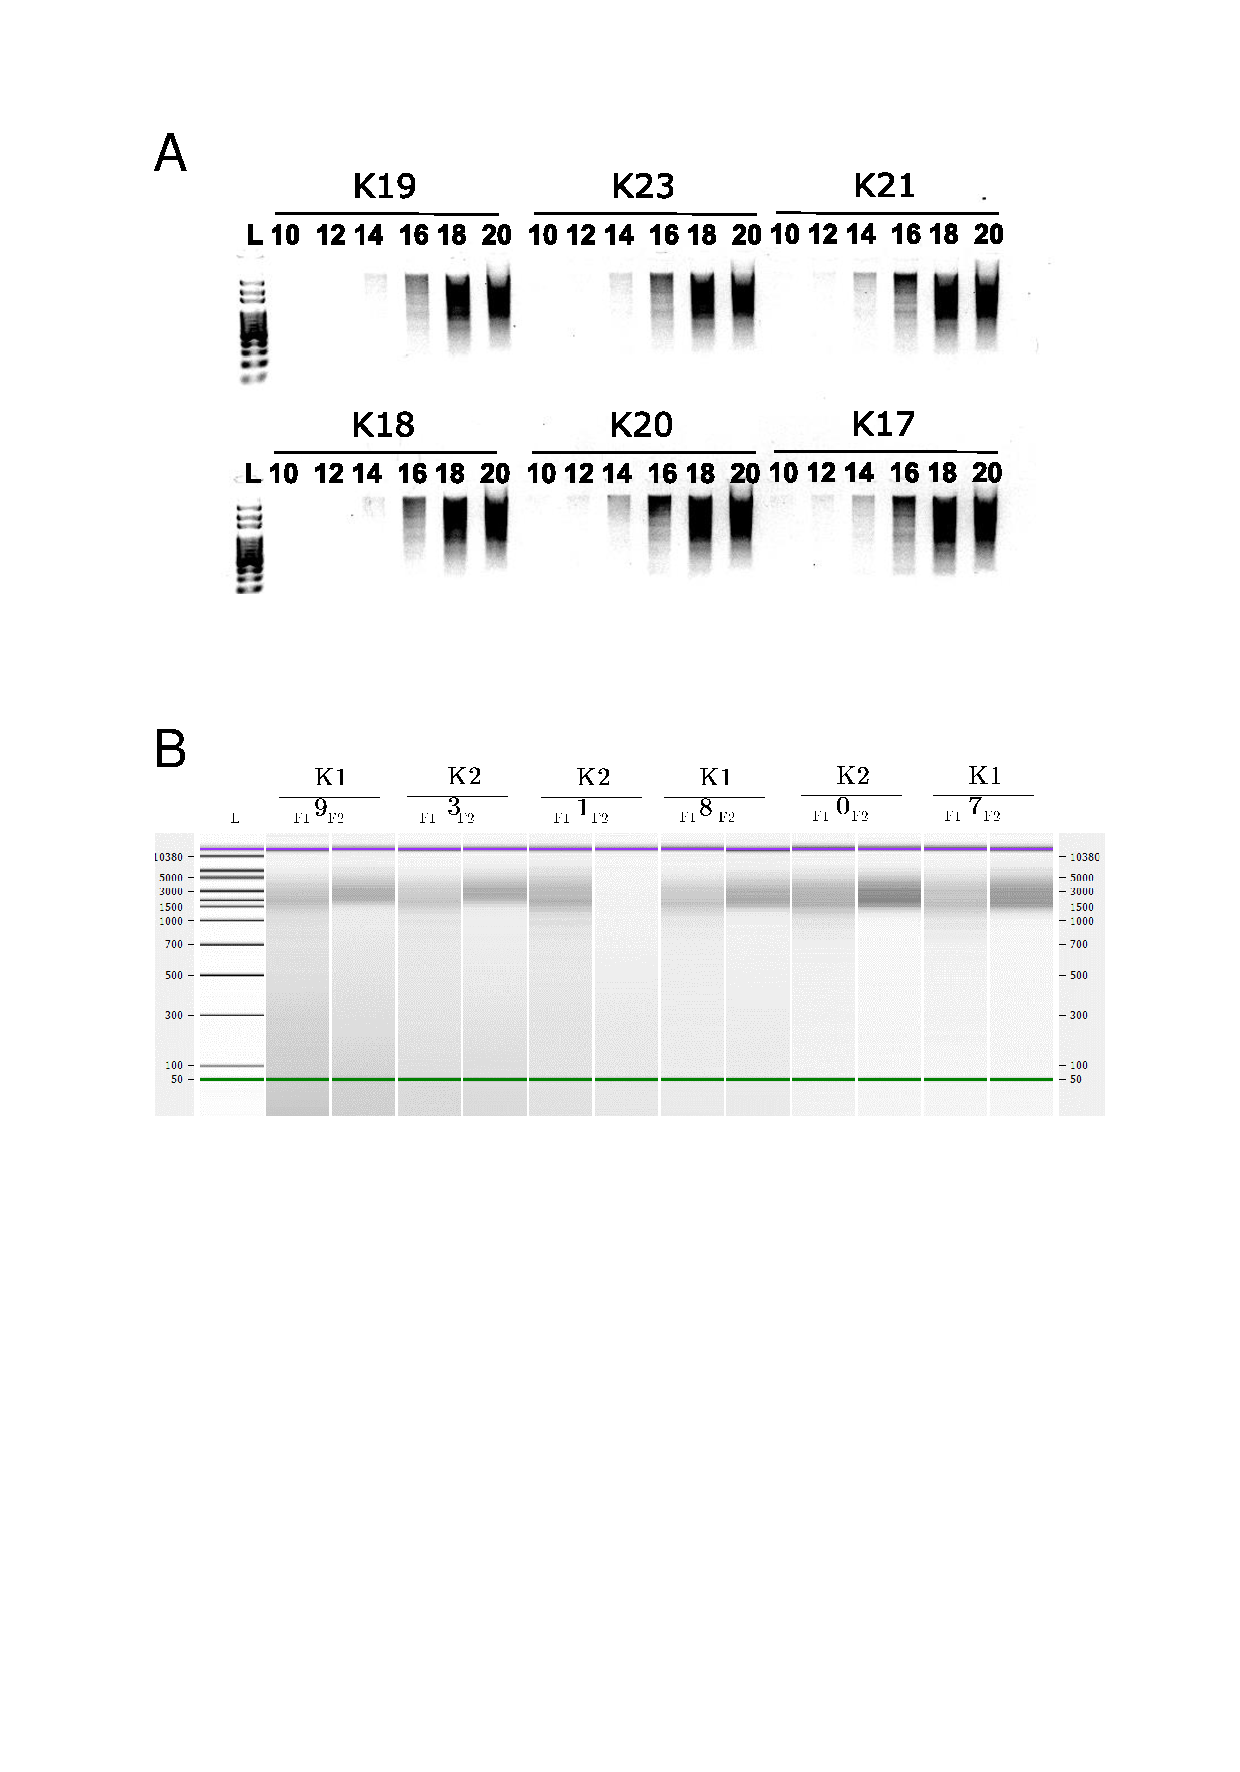
\includegraphics[page=1,trim={0 10cm 0 0cm},clip,scale = 0.75]{Figures/TargetedTranscriptome_LabResults.pdf}
	\captionsetup{width=0.95\textwidth}
	\caption[Iso-Seq Targeted Transcriptome - cDNA amplification and purification]%
	{\textbf{Samples for targeted transcriptome profiling were amplified with 14 PCR cycles: (A)} Analogous to whole transcriptome profiling (\cref{fig:isoseq_whole_pccresults}), samples were amplified using 14 cycles. Ladder (L) denotes to a 100bp DNA ladder. \textbf{(B)} A Bioanalyzer gel of amplified cDNA after purification with 1X (F1) and 0.4X (F2) AMPure beads. Size distribution for each fraction was determined from the start to the end point of the smear. Ladder (L) denotes to a 12kb DNA ladder, whereby the green and purple line represent the lower marker at 50bp and the upper marker at 12kb, respectively.}
	\label{fig:isoseq_targeted_pccresults}
\end{figure}


\begin{figure}[!htp]
	\centering
	\vspace{20pt}
	\includegraphics[page=2,trim={0 17cm 0cm 1cm},clip,scale = 0.75]{Figures/TargetedTranscriptome_LabResults.pdf}
	\captionsetup{width=0.95\textwidth}
	\caption[Iso-Seq Targeted Transcriptome - Target Capture and library preparation]%
	{\textbf{Successful target capture and Iso-Seq library preparation:} Shown are Bioanalyzer electropherograms of \textbf{(A)} Batch 1 (n = 6 samples) after target enrichment and \textbf{(B)} Iso-Seq library preparation, and \textbf{(C)} Batch 2 (n = 9 samples) after target enrichment and \textbf{(D)} Iso-Seq library preparation. 
	\\
	\\
	Illustrating successful target enrichment, we observed peaks that correspond to enriched transcript lengths from genes of interest, which notably differs from the broad peaks seen in whole transcriptome sequencing (\cref{fig:isoseq_whole_bioresults}). Iso-Seq library preparation retained these target transcripts with detection of similar peaks, albeit less pronounced due to a lower cDNA input for Bioanalyzer assays in order to conserve cDNA for maximum sequencing yield.}  
	\label{fig:isoseq_targeted_libresults}
\end{figure}

\begin{figure}[!htp]
	\centering
	\vspace{20pt}
	\includegraphics[page=3,trim={0 17cm 0cm 0cm},clip,scale = 0.75]{Figures/TargetedTranscriptome_ppt.pdf}
	\captionsetup{width=0.95\textwidth}
	\caption[ONT Targeted Transcriptome - Target Capture and library preparation]%
	{\textbf{Successful target capture and ONT library preparation:} Shown in \textbf{(A)} is the TapeStation gel of Batch 2 (n = 9) and Batch 3 (n = 9) after target enrichment and ONT library preparation, and \textbf{B)} is the respective TapeStation electropherogram of Batch 3. 
	\\
	\\
	Illustrating successful target enrichment analogous to \cref{fig:isoseq_targeted_libresults}, we observed peaks that correspond to enriched transcript lengths from genes of interest. Lower cDNA input was used for TapeStation assays to maximise the amount of cDNA available for sequencing. L - Ladder, B2 - Batch 2, B3 - Batch 3.}  
	\label{fig:ONT_targeted_libresults}
\end{figure}

\newpage
\subsection{SMRT sequencing QC and data processing}
Processing of raw reads was performed using the Iso-Seq bioinformatics pipeline (outlined in \cref{section:isoseq_bioinformatics}), and is analogous to the whole transcriptomic dataset processing with the exception of sample demultiplexing using barcode-specific sequences. Briefly, CCS reads were generated from a minimum of 1 pass (\textit{Iso-Seq3 CCS}, v3.4.1) for each batch followed by removal of primers and barcode sequences using \textit{Lima} (v1.9) to generate full-length (FL) reads for each sample. After removal of artificial concatemers reads and trimming of polyA tails using \textit{Iso-Seq3 Refine}, full-length reads were then merged and collapsed to high quality transcripts using \textit{Cupcake} (parameters: -c 0.85 -i 0.95 --dun-merge-5-shorter), and mapped to the mouse reference genome (mm10) using \textit{Minimap2} (v2.17). Full-length Iso-Seq read counts from each individual sample were extracted from \textit{Cupcake's} read\_stat.txt file using the CCS read ID as sample identifier.

\subsection{ONT nanopore sequencing QC and data processing}
QC of raw reads was performed using PycoQC followed by subsequent analysis using the ONT bioinformatics pipeline (details are provided in \cref{section:ont_bioinformatics}). Briefly, raw reads were basecalled using \textit{Guppy} (v4.0) and reads with Phred (Q) < 7 were filtered. Primers and ONT adapters were then removed using \textit{Porechop} (v0.2.4) to generate full-length reads for each sample. After trimming of polyA tails using \textit{Cutadapt} (v2.9), full-length reads were then mapped to the reference mouse genome (mm10) using \textit{Minimap2} (v2.17, parameters: "-ax splice"). Owing to the high error rate of ONT nanopore sequencing, artefactual non-canonical splice junctions from mapped reads were corrected with \textit{Transcript Clean}. Corrected reads were then processed using \textit{TALON} (v5.0) for annotation, quantification and filtering for intrapriming (--maxFracA = 0.5). Novel transcripts were only retained if >5 full-length reads and detected in >2 samples. \textit{TALON} was chosen as the preferred tool for ONT processing after trialling multiple tools (more details are provided in \textbf{Appendix} \textbf{\ref{ONT_Bioinformatics_appendix}}). 

\subsection{Comparison of Iso-Seq and ONT datasets}
The Iso-Seq targeted dataset (n = 24 samples) was examined with other datasets using \textit{Gffcompare}; such datasets included Iso-Seq-derived transcripts identified from whole transcriptome profiling (n = 12 samples, \cref{tab:isoseq_wholerun_result}, Iso-Seq whole dataset) and ONT-derived transcripts from targeted transcriptome profiling (n = 18 samples, \cref{tab:mouse_samples_sequenced}, ONT targeted dataset). For a fair comparison, Iso-Seq whole dataset was re-annotated with \textit{SQANTI3} with no splice junction filtering from short-read RNA-Seq data, and only transcripts derived from matched samples were used for comparison. Conversely, all processed but unfiltered ONT reads were used for a comprehensive comparison between the two technologies with Iso-Seq derived transcripts as reference. 

\begin{figure}[htp]
	\centering
	\includegraphics[page=16,trim={0cm 8cm 0cm 0cm},clip,scale = 0.8]{Figures/ProjectDevelopment_Figures}
	\captionsetup{width=0.95\textwidth,singlelinecheck=off}
	\caption[ONT Targeted Bioinformatics Pipeline]%
	{\textbf{ONT Targeted Bioinformatics Pipeline:} Shown is a detailed bioinformatics pipeline for processing ONT reads from targeted transcriptome profiling after sequencing of the rTg4510 cortex (S\textsubscript{n}) on two flow cells (referred as Batch 2 and Batch 3 of the Iso-Seq targeted dataset, summarised in \cref{tab:mouse_samples_sequenced}). Supplementing \cref{fig:ONT_PacBio_bioinformatics}, raw ONT reads from each flow cell were processed and demupliplexed using \textit{Porechop} to generate sample-specifici reads, which were subsequently processed independently for collapse and transcript quantification. Samples from both batches were then merged into one dataset, while retaining sample-specific transcript expression. 
	}
	\label{fig:ONT_Targeted_bioinformatics}
\end{figure}

\subsection{Merged annotation and quantification}
\label{ch6: methods_quantification}
For a comprehensive characterisation of the target genes enriched in the rTg4510 cortex, full-length transcripts from the Iso-Seq and ONT targeted datasets were merged using \textit{Gffcompare} (depicted in \cref{fig:Targeted_bioinformatics_pipeline}). A custom python script ("identify\_common\_targeted\_transcripts.py") was then applied to: i) identify transcripts detected using both PacBio Iso-Seq and ONT nanopore sequencing, which were defined as a complete exact match in \textit{Gffcompare} output (class code: "="), ii) retain ONT-derived novel transcripts that did not pass \textit{TALON} filtering (>5 reads and detected in >2 samples), but were detected in the Iso-Seq targeted dataset, iii) retain all transcripts unique to the Iso-Seq targeted dataset given the stringent processing and high accuracy of Iso-Seq reads, and iv) generate an abundance file for each sample and transcript, either tabulating counts from \textit{Cupcake} for Iso-Seq-derived-transcripts, counts from \textit{TALON} for ONT-derived-transcripts or the count summation for commonly detected transcripts. The merged dataset was then annotated with \textit{SQANTI3} in combination with mouse reference gene annotations (mouse GENCODE, vm22), FANTOM5 CAGE peaks and \textit{STAR}-aligned RNA-Seq junctions. Isoform were subsequently classified as either FSM, ISM, NIC, NNC, antisense, fusion, and intergenic (described in \cref{section: sqanti_annotations}). Isoforms classified as ISM with 3'fragment were assumed to be partial 5'RNA degraded products and removed. 

\begin{figure}[htp]
	\centering
	\includegraphics[page=5,trim={0.5cm 7cm 0cm 0cm},clip,scale = 0.8]{Figures/TargetedTranscriptome_LabResults}
	\captionsetup{width=0.95\textwidth,singlelinecheck=off}
	\caption[Bioinformatics Pipeline for merging targeted Iso-Seq and ONT datasets]%
	{\textbf{Bioinformatics Pipeline for merging targeted Iso-Seq and ONT datasets}. Shown is a outline of the bioinformatics pipeline for processing Iso-Seq reads and ONT reads 1D reads from the targeted transcriptome profiling of the mouse cortex. 
	}
	\label{fig:Targeted_bioinformatics_pipeline}
\end{figure}

\newpage
\subsection{Characterisation of AS events and transcript visualisation}
To date, current tools for assessing alternative splicing events were developed for short-read RNA-Seq data and fail to capture the connectivity and complexity of long-read-derived isoforms, particularly in targeted transcriptome profiling where deep sequencing coverage is achieved. A custom python script ("annotate\_common\_targeted\_transcripts.py") was therefore developed to accurately assess the occurrence of alternative splicing events by comparing splice sites (exon) coordinates between long-read-derived transcripts and reference transcripts (mm10) (depicted in \cref{fig:Targeted_bioinformatics_pipeline}). Common alternative splicing events such as alternative first exons (AF), alternative last exons (AL), alternative 5' splice sites (A5), alternative 3' splice sites (A3), intron retention (IR) and exon skipping (ES) were assessed (depicted in \cref{fig:AS_events}). Alternative 5' and 3' splice sites were defined as splice sites differing by more than 10bp from the known splice site, and an intron was considered retained if the exon splice site differed by more than 100bp from the known splice site (depicted in \cref{fig:Targeted_isoforms_annotate}). Other regulatory mechanisms such as alternative transcription initiation (defined by alternative TSS) and termination (defined by alternative TSS), and the presence of novel exons, were also evaluated. 

Open reading frames were predicted using the CPAT program (v3.0.2) under default parameters, and transcripts with coding potential score >0.44 (recommended threshold) were predicted as protein-coding. Isoforms were predicted for nonsense-mediated decay if distance between predicted open read frame and last exon-exon junction was >50bp. Finally, a separate custom python script ("colour\_common\_targeted\_transcripts.py") was applied to colour transcripts by coding potential (green for protein coding, red for non-protein coding) and shade by abundance. Isoforms were then grouped by splicing patterns and visualised using the UCSC genome browser. 

\begin{figure}[htp]
	\centering
	\includegraphics[page=7,trim={0cm 5cm 0cm 0cm},clip,scale = 0.75]{Figures/TargetedTranscriptome_LabResults}
	\captionsetup{width=0.95\textwidth,singlelinecheck=off}
	\caption[Characterisation of isoforms detected in targeted transcriptome profiling]%
	{\textbf{Characterisation of isoforms detected in targeted transcriptome profiling:} \textbf{(A)} Reference transcripts were "flattened" to obtain splice site coordinates. \textbf{(B)} Exon-level comparison of long-read-derived transcripts and reference transcripts was then performed by comparing splice site coordinates to assess occurrence of alternative splicing sites. Splice sites differing <10bp ("wobble") were considered identical, >10bp as truncation, >10bp but <100bp as extension ,and >100bp as intron retention.  
	}
	\label{fig:Targeted_isoforms_annotate}
\end{figure}

\begin{figure}[htp]
	\centering
	\includegraphics[page=8,trim={0cm 1cm 0cm 0cm},clip,scale = 0.75]{Figures/TargetedTranscriptome_LabResults}
	\captionsetup{width=0.95\textwidth,singlelinecheck=off}
	\caption[Visualising isoforms by coding, abundance and NMD status]%
	{\textbf{Visualising isoforms by coding, abundance and NMD status:} \textfbf{(A)} Open reading frames were determined using \textit{CPAT} and \textbf{(B)} isoforms were subsequently coloured by protein coding potential (green for coding, red for non-coding, and gray for no open reading frame) and shaded by abundance (described in \cref{ch6: methods_quantification}) \textbf{(C)} A schematic figure illustrating approach for predicting nonsense-mediated decay (NMD). ORF - Open Reading Frame. 
	}
	\label{fig:Targeted_isoforms_cpat}
\end{figure}

\subsection{Differential analysis}
Differential expression analysis was performed with \textit{tappAS} using full-length read counts from Iso-Seq and nanopore sequencing (fully described in \cref{ch3_tappas_explained}). Briefly, \textit{tappAS} filters out lowly-expressed isoforms, normalises read counts using TMM approach and performs differential expression analysis using \textit{maSigPro}\cite{Conesa2006,Nueda2014,Conesa2017} to elucidate effects for both genotype and age. 

\newpage
\section{Results}
\subsection{Iso-Seq run performance and sequencing metrics}
Following Iso-Seq library preparation and SMRT sequencing, we generated a total of 62.8Gb (mean = 20.9Gb, s.d = 2.84Gb, range = 19.25Gb - 24.2Gb, \cref{tab:targeted_mouse_run_output}). While the sequencing yield was comparable to whole transcriptome profiling (\cref{tab:isoseq_wholerun_result}), the run performance varied across the three Iso-Seq targeted datasets, particularly between Batch 1 (n = 6 samples) and Batches 2 (n = 9 samples), 3 (n = 9 samples), which were sequenced pre- and post-Covid-19 lockdown respectively. The run performance metrics for Batch 1 were optimal (\cref{tab:targeted_mouse_run_output}). Conversely, Batches 2 and 3 had a poor loading rate (Batch 1 P1:  71\%, Batch 3 P1: 38.1\%) with sequencing yields that were comparable to Batch 1, despite containing more samples. We suspect that this low run performance was likely a result of sample degradation, given samples were stored in -20\textdegree C for >9 months (due to Covid-19 lockdown) before sequencing. 

Following the Iso-Seq bioinformatics pipeline, raw reads were processed and clustered to unique consensus transcripts, which were then mapped to the mouse reference genome. A total of 966K CCS reads (mean = 332K, s.d = 126K, range =  221K - 469K) and 930K FLNC reads (mean = 310K, s.d = 77.7K, range = 2556K - 399K) were successfully generated (\cref{fig:isoseq_targeted_run_output}\textbf{A}). Where there was evident difference in the number of CCS reads obtained for Batch 1 and Batches 2,3 - a reflection of the run performance - Batches 2 and 3 had a significantly greater coverage of target genes than Batch 1 (\cref{fig:isoseq_targeted_rate}). These results indicate that the poorer run performance and subsequent lower sequencing yield of Batches 2 and 3 were compensated by a bigger sample size, generating more full-length reads associated to target genes. In contrast, the better run performance but lower sample size of Batch 1 resulted in quicker saturation of target genes and generation of more full-length reads associated to off-target genes. 

Finally, we noted that the number of full-length transcripts obtained per sample varied within each batch (\cref{fig:isoseq_targeted_run_output}\textbf{B}), despite pooling of samples with equal molarity during library preparation. This variability was not associated with RIN (corr = 0.147, P = 0.492, Spearman's rank). However, no significant difference in the number of full-length transcripts was observed between WT and TG across the runs (Wilcoxon rank sum test, W = 73, P = 0.977, \cref{fig:isoseq_targeted_run_output}\textbf{C}). 


\begin{table}[]
	\captionsetup{width=1.0\textwidth}
	\caption[Iso-Seq sequencing yield for targeted transcriptome profiling of rTg4510 mouse cortex]%
	{\textbf{Iso-Seq sequencing yield for targeted transcriptome profiling of the rTg4510 mouse cortex:} rTg4510 cortex (n = 9 WT, n = 9 TG) was sequenced using the Iso-Seq approach on 3 runs (Batch 1, 2 and 3) after multiplexing and enrichment of 20 AD-associated genes. Further details on evaluation of the performance of Iso-Seq sequencing runs are provided in \cref{sec: Isoseq_run_performance}. K - Thousand, Pol - Polymerase. N50 is defined as the sequence length of the shortest read at 50\% of all reads}
	\label{tab:targeted_mouse_run_output}
	\centering
	\setlength\tabcolsep{6pt} %reduced margin size in table
	\begin{tabularx}{\textwidth}{cccccccccc}
		\toprule
		\multirow{3}{*}{Runs} &
		\multirow{3}{*}{\begin{tabular}[c]{@{}c@{}}Total \\ Bases\\ (Gb)\end{tabular}} &
		\multirow{3}{*}{\begin{tabular}[c]{@{}c@{}}Polymerase\\  Reads (K)\end{tabular}} &
		\multicolumn{4}{c}{Read Length (kB)} &
		\multicolumn{3}{c}{Productivity} \\ \cmidrule(l){4-10} 
		&&&
		\multicolumn{2}{c}{Polymerase} &
		\multicolumn{2}{c}{Subread} &
		\multirow{2}{*}{P0} &
		\multirow{2}{*}{P1} &
		\multirow{2}{*}{P2} \\
		&&&
		Mean & N50 & Mean & N50 &&&
		\\ \midrule
		Batch 1 & 24.2 & 712 & 34.0 & 70.5 &	1.4 & 1.85 &
		\begin{tabular}[c]{@{}c@{}}4.62\% \\ (46613)\end{tabular} &
		\begin{tabular}[c]{@{}c@{}}71.58\% \\ (722026)\end{tabular} &
		\begin{tabular}[c]{@{}c@{}}24.76\% \\ (249707)\end{tabular} \\
		Batch 2 &
		&&&&&&&
		&
		\\
		Batch 3 &	19.3 &	384 &	50.5 &	100 &	1.6 &
		2.02 &
		\begin{tabular}[c]{@{}c@{}}18.68\% \\ (189549)\end{tabular} &
		\begin{tabular}[c]{@{}c@{}}38.11\% \\ (386743)\end{tabular} &
		\begin{tabular}[c]{@{}c@{}}43.56\% \\ (442054)\end{tabular} \\ \bottomrule
	\end{tabularx}
\end{table}


\begin{figure}[!htp]
	\begin{center}
		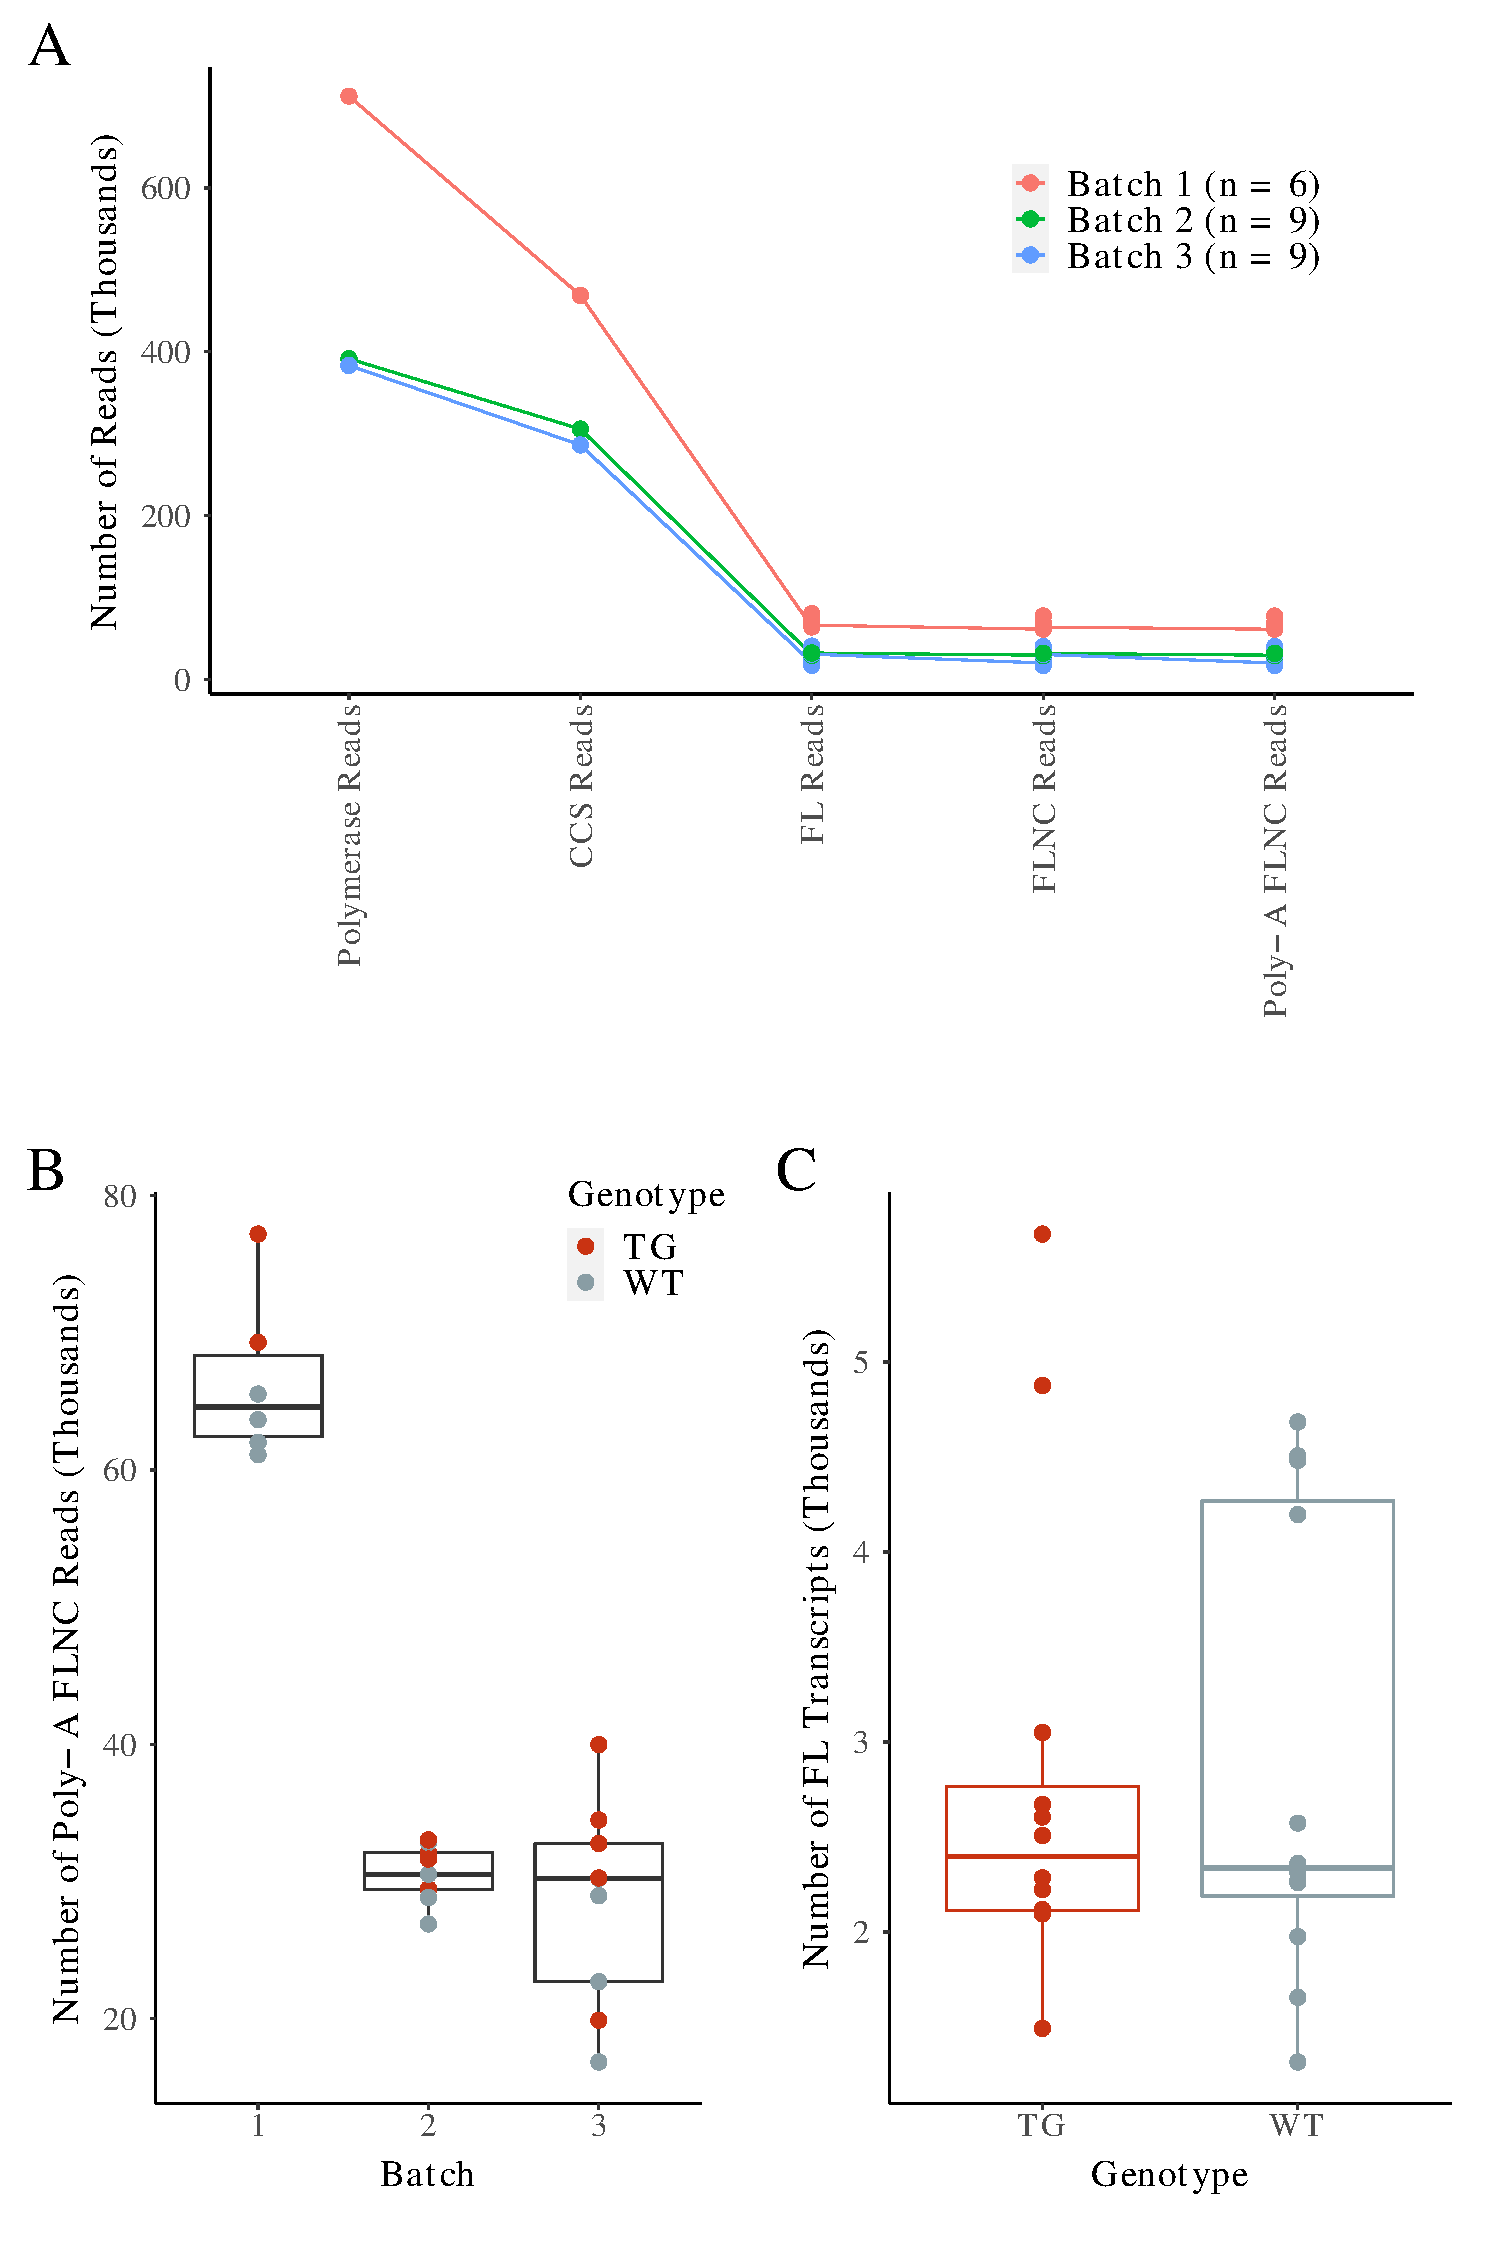
\includegraphics[page=1,trim={0 1cm 0 0},clip,scale = 0.55]{Figures/TargetedTranscriptome.pdf}
	\end{center}
	\captionsetup{width=0.95\textwidth}
	\caption[Targeted Transcriptome Iso-seq run performance]%
	{\textbf{Despite batch variability in Iso-Seq targeted datasets, no difference was reported in the number of FL transcripts between WT and TG mice:} \textbf{(A)} The number of reads generated through the Iso-Seq bioinformatics pipeline from initial generation of CCS reads, to FL reads with primer removal, and poly-A FLNC reads with removal of artificial concatemers and trimming of poly(A) tails. Samples were multiplexed and sequenced in three runs (Batch 1, 2 and 3). Shown is a \textbf{(B)} box-plot of the number of poly-A FLNC reads by batch and genotype and \textbf{(C)} box-plot of the final number of FL transcripts by genotype. CCS - Circular Consensus Sequence, FLNC - Full-Length Non-Concatemer, FL - Full-Length, WT - Wild-type, TG - Transgenic}
	\label{fig:isoseq_targeted_run_output}
\end{figure}

\begin{figure}[!htp]
	\centering
		\includegraphics[page=2,trim={0 25cm 0 0},clip,scale = 0.55]{Figures/TargetedTranscriptome.pdf}
	\captionsetup{width=0.95\textwidth}
	\caption[On-Target rate of Iso-Seq targeted transcriptome profiling]%
	{\textbf{Higher coverage of target genes in Batches 2 and 3 due to more samples multiplexed and sequenced:} Shown is a box-plot of the on-target rate, defined as the proportion of mapped transcripts associated with target genes (AD-associated genes) with overlapping sequences to at least one target probe. Of note, a difference in the on-target rate between WT and TG in Batch 1 is a likely reflection of the sample variability in sequencing (\cref{fig:isoseq_targeted_run_output}\textbf{B}). WT - Wild-type, TG - Transgenic.}
	\label{fig:isoseq_targeted_rate}
\end{figure}

\newpage
\subsection{Iso-Seq targeted transcriptome profiling approach detects many novel, rare isoforms annotated to AD-associated genes}
\label{ch6: wholevstargeted}
Following stringent quality-control and filtering of technical artefacts, we detected 19,659 isoforms in the Iso-Seq targeted dataset of which 2,015 isoforms (10.2\%) were annotated to 20 AD-associated genes enriched in the rTg4510 cortex (n = 12 WT, n = 12 TG). This was in stark contrast to the whole transcriptome profiling dataset, where we detected 175 isoforms (0.25\% of total number of isoforms detected from whole transcriptome profiling) annotated to the same AD-associated genes, highlighting the success of targeted profiling for deep coverage of target genes. As expected, target enrichment and sequencing of matched samples (n = 6 WT, 6 TG, \cref{tab:whole_phenotype}) detected many more AD-associated transcripts than the whole transcriptome profiling approach (\cref{fig:targeted_vs_whole}\textbf{A}, Iso-Seq whole dataset: n = 46 unique isoforms, Iso-Seq targeted dataset = 658 unique isoforms, Iso-Seq Whole and targeted dataset = 221 isoforms). The majority of these isoforms unique to the Iso-Seq targeted dataset were novel (\cref{fig:targeted_vs_whole}\textbf{B}, n = 525 isoforms, 79.8\%) as NIC (n = 218 isoforms, 33.1\%) and NNC (n = 307 isoforms, 46.7\%), and less abundant (\cref{fig:targeted_vs_whole}\textbf{D}), highlighting the greater sensitivity of the targeted profiling approach to detect the novel, rarer transcripts. Strikingly, the whole transcriptome profiling approach detected all the target genes with the exception of \textit{Trpa1}, the least expressed target gene in the mouse cortex (\cref{tab:target_genes_description}), which suggests that the gene sensitivity with 5.6 million CCS reads (n = 12 samples) using the Iso-Seq whole transcriptome profiling approach was capped between 0.1 TPM (mouse cortex \textit{Trpa1} expression) and 0.5 TPM (mouse cortex \textit{Rhbdf2} expression, the second least expressed target gene). Given that our whole Iso-Seq datasets approached saturation particularly at the gene level (\cref{fig:isoseq_whole_rarefaction}\textbf{A}), it is unlikely that we would have been to detect \textit{Trpa1} with more samples using the whole transcriptome profiling approach.

Further comparison of the isoform landscape of AD-associated genes in the Iso-Seq whole and targeted datasets revealed similar distribution of isoform length (Iso-Seq whole dataset: mean = 2.67kb, s.d = 1.6kb, range = 300bp - 10.3kb, Iso-Seq targeted dataset: mean = 2.4kb, s.d = 1.2kb, range = 140bp - 10.3kb; Mann-Whitney-Wilcoxon test: W = 1.91 x 10\textsuperscript{6}, P = 0.068) and number of exons (Iso-Seq whole dataset: mean = 12.9, s.d = 9.6, range - 1 - 50; Iso-Seq targeted dataset: mean = 11.7, s.d = 7.9, range = 1 - 50; Mann-Whitney-Wilcoxon test: W = 1.86 x 10\textsuperscript{6}, P = 0.22). Drawing parallels to the isoform landscape of the global transcriptome, approximately half of the isoforms identified in Iso-Seq targeted dataset were novel (n = 919 isoforms, 45.6\%) as NIC (n = 485, 24.1\%) and NNC (n = 434 isoforms, 21.5\%) (\cref{fig:isoseq_targeted_finalnumberiso}\textbf{A}), with the remaining half identified as known and predominantly ISM (n = 913, 45.3\%). However, AD-associated isoforms in Iso-Seq targeted dataset were less enriched near CAGE peaks from the FANTOM5 dataset (median distance from CAGE peak = 335 bp, 646 transcripts located within 50bp of a CAGE peak) than those in Iso-Seq whole dataset (median distance from CAGE peak = 2 bp, 122 transcripts (69.7\%) located with 50bp of a CAGE peak), and were located further to annotated transcription start sites (Iso-Seq targeted dataset: median distance = 808bp, Iso-Seq whole dataset: median distance = 8bp) and transcription termination sites (Iso-Seq targeted dataset: median distance = 2bp, Iso-Seq whole dataset: median distance = 1bp). 

Generating highly parallel RNA-Seq data on the same samples (n = 24 samples, total number of uniquely mapped reads = 360 million), we further found that a vast majority of these isoforms had no RNA-Seq support at the junction (n = 1658 isoforms, 82.2\%). Given the stringent process of the Iso-Seq bioinformatics pipeline and target enrichment, this is a likely reflection of the low coverage of RNA-Seq reads to comprehensively span these novel junctions. However, a strong correlation between gene-level expression was observed across both methods (n = 20 genes, corr = 0.86, P < 2.23 x 10\textsuperscript{-308}, \cref{fig:isoseq_targeted_finalnumberiso}\textbf{B}). 

Finally, we observed a high off-target rate of Iso-Seq targeted experiments with detection of isoforms (n = 17,644, 89.8\%) that were not associated with target genes. Comparison with the whole Iso-Seq datasets using matched samples (n = 12, n = 7,925 off-target isoforms, 89.8\%) revealed that the overwhelming majority of these isoforms (n = 7,418, 93.6\% off-target isoforms) were also detected in the whole Iso-Seq dataset. These isoforms were more abundant than isoforms unique to the whole Iso-Seq dataset and isoforms associated to target genes (\cref{fig:targeted_vs_whole}\textbf{C}), suggesting that capture of off-target genes is predominantly driven by abundance rather than sequence homology to target genes (off-target binding).  

\begin{figure}[!htp]
	\centering
	\includegraphics[page=3,trim={0 1.5cm 0 0cm},clip,scale = 0.50]{Figures/TargetedTranscriptome.pdf}
	\label{fig:targeted_vs_whole}
	\captionsetup{width=0.95\textwidth}
	\caption[Comparison of whole transcriptome vs targeted Iso-Seq transcriptome profiling]%
	{\textbf{Iso-Seq targeted approach detected many more novel and rarer transcripts than whole transcriptome profiling of the mouse cortex}. Shown is the \textbf{(A)} number of isoforms per target gene that were uniquely detected using the Iso-Seq targeted transcriptome profiling approach ("Targeted"), uniquely detected in the Iso-Seq whole transcriptome profiling approach ("Whole") and in both datasets ("Both"), and the \textbf{(B)} number of isoforms in the Iso-Seq targeted approach stratified by structural category. \textbf{(C)} A box-plot of the full-length read counts of isoforms associated to target and non-target genes in the Iso-Seq whole and \textbf{(D)} targeted datasets. Target genes refer to the panel of 20 AD-associated genes that were enriched for targeted sequencing. Only transcripts from matched samples were compared. FSM - Full Splice Match, ISM - Incomplete Splice Match, NIC - Novel In Catalogue, NNC - Novel Not in Catalogue.}
\end{figure}

\begin{figure}[!htp]
	\begin{center}
		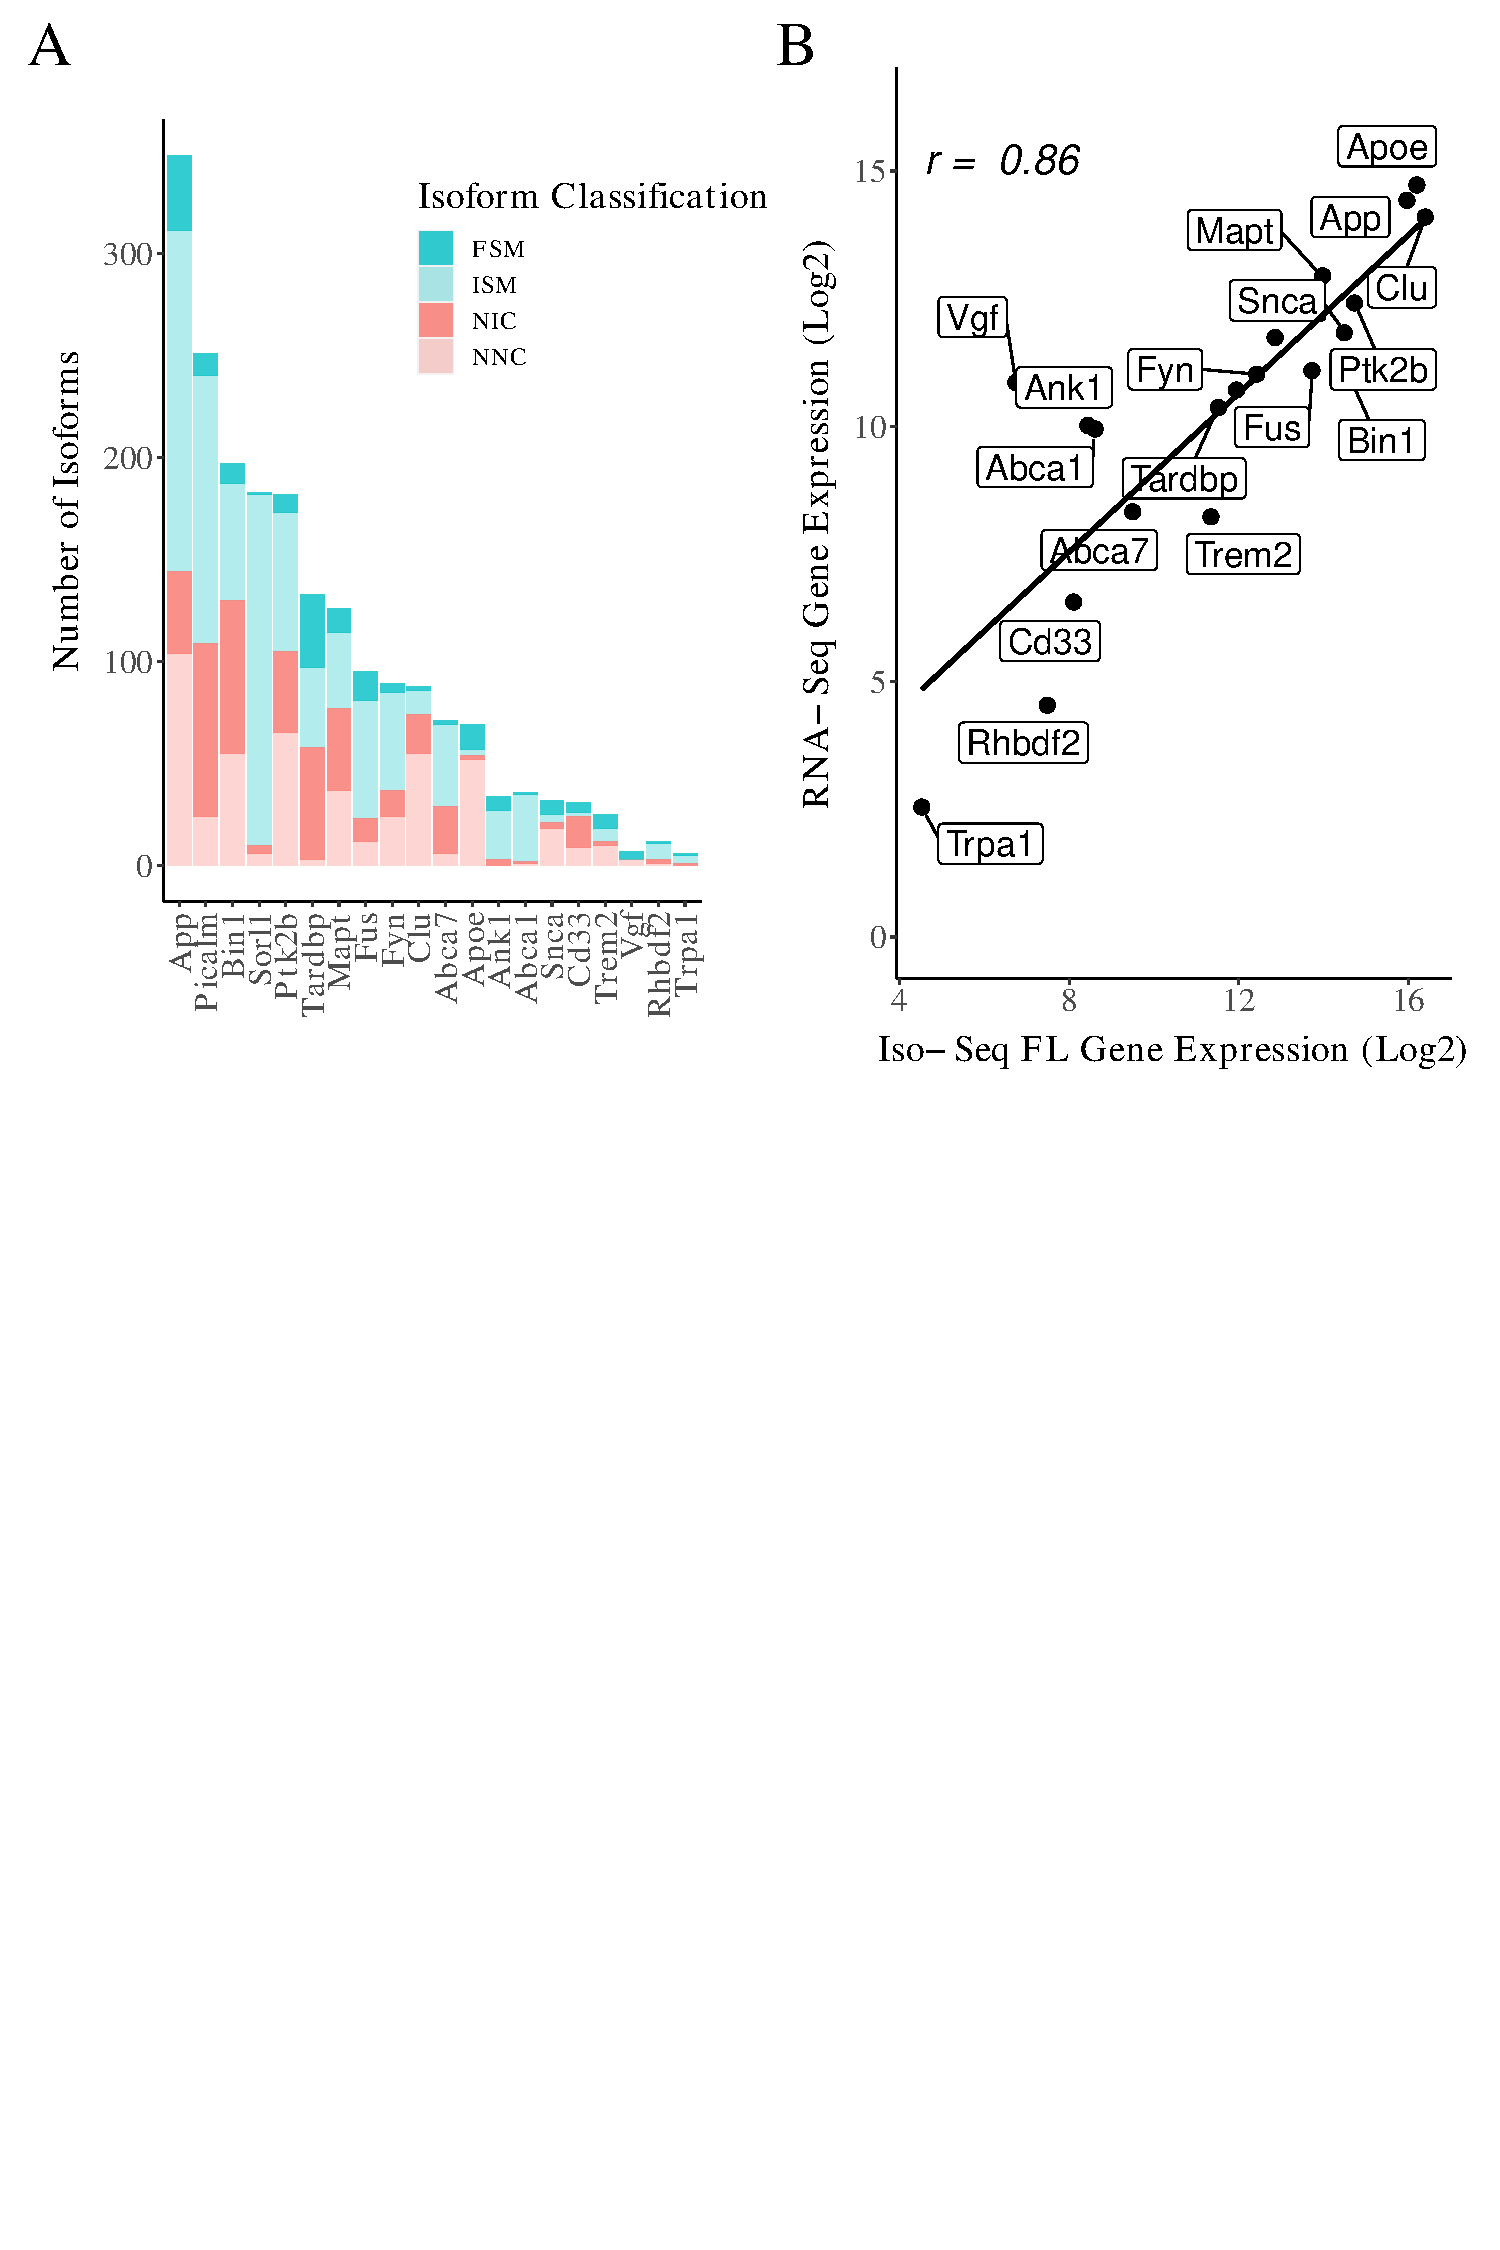
\includegraphics[page=1,trim={0 20cm 0 0cm},clip,scale = 0.60]{Figures/ONTvsIsoSeq.pdf}
	\end{center}
	\captionsetup{width=0.95\textwidth}
	\caption[Wide isoform diversity in AD-associated genes from Targeted Sequencing in mouse cortex]%
	{\textbf{Wide isoform diversity observed in AD-associated genes with many novel isoforms detected}. \textbf{(A)} Shown is the number of isoforms detected per target gene from the Iso-Seq targeted dataset, classified by novel and known, after sequential processing and filtering in the bioinformatics Iso-Seq pipeline. Novel isoforms refer to isoforms that are not known in current existing annotations. \textbf{(B)} A strong correlation was observed between Iso-Seq and RNA-Seq gene expression. Iso-Seq gene expression was determined from the summation of full-length read counts of associated transcripts, whereas RNA-Seq gene expression was deduced from the normalised \textit{DESeq} counts of aligned RNA-Seq reads to reference genome\cite{Castanho2020}.}
	\label{fig:isoseq_targeted_finalnumberiso}
\end{figure}


\newpage
\subsection{ONT run performance and sequencing metrics}
\label{ch6: ont_run_performance}
Following library preparation and nanopore sequencing on a subset of samples (n = 8 WT, n = 10 TG, \cref{tab:mouse_samples_sequenced}), a total of 28.54M reads (39.68Gb) were generated across two flow cells (Batch 2 and Batch 3) and a total of 22.8M (80\%) reads were successfully basecalled using \textit{Guppy} (\cref{tab:ont_targetedrun_output}). Although both flow cells achieved good sequencing yield with similar read lengths, Batch 3 had a significantly greater throughput, generating more basecalled reads (pre-filter: Batch 2: 12.3M and Batch 3: 16.3M; post-filter: Batch 2: 9.68 (78.8\%); Batch 3: 13.13M (80.7\%). Evaluation of the run performance and QC using \textit{PycoQC} revealed that this disparity was the result of lower sequencing channel activity in Batch 2 with a number of inactive pores (\cref{fig:ont_targetedseq_channel}). The number of bases generated over the course of the run was thus significantly lower in Batch 2 than in Batch 3 (\cref{fig:ont_targetedtime_performance}).  


\vspace{1cm}
\begin{table}[!htp]
	\captionsetup{width=0.95\textwidth}
	\caption[Run Yield Output from Targeted Transcriptome Nanopore Sequencing of Tg4510]%
	{\textbf{Comparable run performance and yield output from Targeted Nanopore sequencing of Tg4510}. A subset of samples (n = 18) were also prepared for sequencing on the ONT MinION using two separate flow cells over 48hours (Batch 2: WT = 4, TG = 5 samples; Batch 3: WT = 4, TG = 5 samples). Following the ONT bioinformatics pipeline, raw ONT reads were basecalled and filtered by read accuracy (Phred, Q > 7). Active channels refer to the total number of channels that were detected with sequencing activity over the course of the run. N50 refers to the sequence length at which 50\% of reads are sized at or over. Gb - Gigabases, kb- kilobases, M - Million}
	\label{tab:ont_targetedrun_output}
	\centering
	\setlength\tabcolsep{4pt} %reduced margin size in table
	\begin{tabular}{@{}cccccccccc@{}}
		\toprule
		\multirow{3}{*}{Runs} &
		\multirow{3}{*}{\begin{tabular}[c]{@{}c@{}}Active\\  channels\end{tabular}} &
		\multicolumn{2}{c}{Basecalled reads} &
		\multicolumn{6}{c}{Filtered basecalled   reads} \\ \cmidrule(l){3-10} 
		&
		&
		\multirow{2}{*}{\begin{tabular}[c]{@{}c@{}}Total \\ Bases\\  (Gb)\end{tabular}} &
		\multirow{2}{*}{\begin{tabular}[c]{@{}c@{}}Number \\ (M)\end{tabular}} &
		\multirow{2}{*}{\begin{tabular}[c]{@{}c@{}}Total\\  Bases \\ (Gb)\end{tabular}} &
		\multirow{2}{*}{\begin{tabular}[c]{@{}c@{}}Number\\  (M)\end{tabular}} &
		\multicolumn{3}{c}{Read Length (bp)} &
		\multirow{2}{*}{\begin{tabular}[c]{@{}c@{}}Mean \\ Read\\  Quality\end{tabular}} \\ \cmidrule(lr){7-9}
		&
		&
		&
		&
		&
		&
		Mean &
		N50 &
		\begin{tabular}[c]{@{}c@{}}Longest \\ Read (kb)\end{tabular} &
		\\ \midrule
		Batch 2 &
		479 &
		16.9 &
		12.2 &
		14.2 &
		\begin{tabular}[c]{@{}c@{}}9.68 \\ (78.8\%)\end{tabular} &
		1,478 &
		1,779 &
		19.1 &
		10.2 \\
		Batch 3 &
		425 &
		22.8 &
		16.2 &
		19.41 &
		\begin{tabular}[c]{@{}c@{}}13.1 \\ (80.7\%)\end{tabular} &
		1,468 &
		1,813 &
		20.5 &
		9.9 \\ \bottomrule
	\end{tabular}
\end{table}

\begin{figure}[htp]
	\begin{center}
		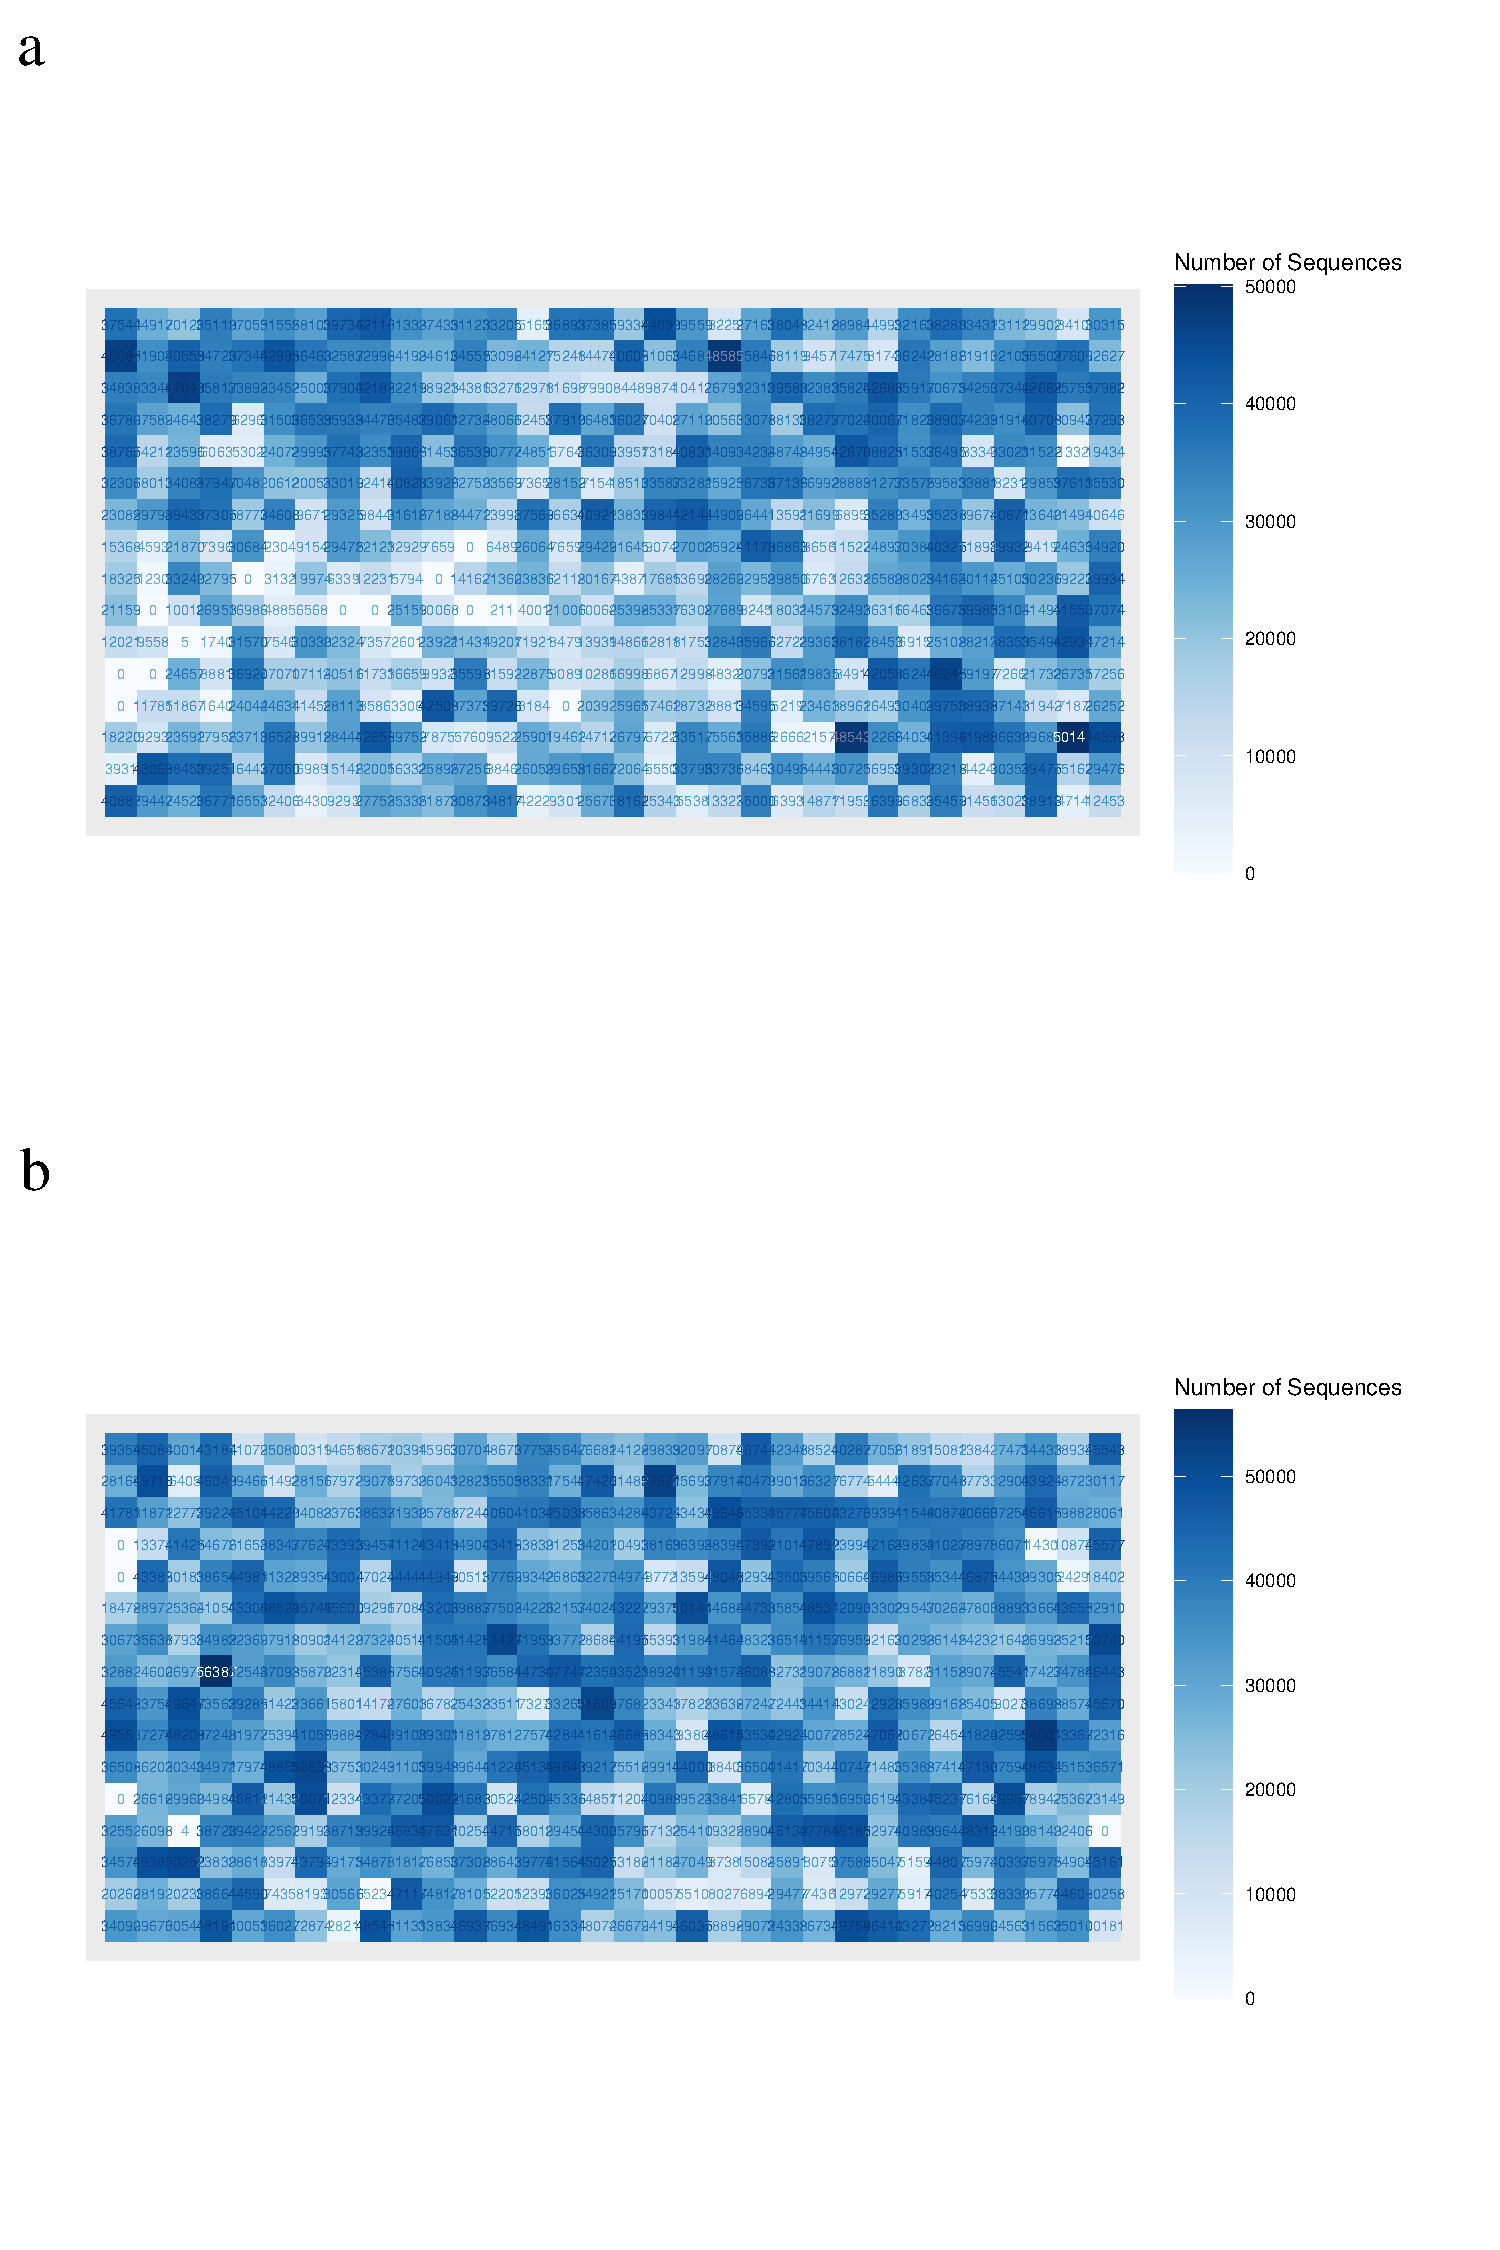
\includegraphics[page=1,trim={0 13cm 0 0},scale = 0.45]{Figures/ONTTargetedTranscriptome.pdf}
	\end{center}
	\captionsetup{width=0.95\textwidth}
	\caption[ONT sequencing channel activity for targeted transcriptome profiling of rTg4510 cortex]%
	{\textbf{ONT sequencing channel activity for targeted transcriptome profiling of rTg4510 cortex:} Shown is a spatial heatmap representation of channel productivity for \textbf{(A)} Batch 2 (sequencing yield = 16.9Gb) and \textbf{(B)} Batch 3 (sequencing yield = 22.8Gb). Each square is a channel that contains 4 nanopore nanopore, and the productivity is determined by the number of DNA sequences (represented here with a colour density from white to dark blue) that translocates through each pore in the duration of a given run. A contrast in activity can be seen across both runs: a concentrated patch of inactive channels(white box, 0 reads translocated through pore of interest) in the Batch 2 run vs more active channels (dark blue, >50,000 reads translocated through pore of interest) in the Batch 3 run. Similar amounts of cDNA were loaded into the flow cells (Batch 2: 540ng, Batch 3: 500ng)}
	\label{fig:ont_targetedseq_channel}
\end{figure}

\begin{figure}[htp]
	\begin{center}
		\includegraphics[page=2,,trim={0 0cm 0cm 10cm},clip, scale = 0.45]{Figures/ONTTargetedTranscriptome.pdf}
	\end{center}
	\captionsetup{width=0.95\textwidth}
	\caption[ONT temporal run performance for targeted transcriptome profiling]%
	{\textbf{ONT temporal run performance for targeted transcriptome profiling:} Shown are time-series plots with the \textbf{(A)} number of bases generated per hour over the course of the run for Batch 2 and \textbf{(B)} Batch 3, and \textbf{(C)} the reads generated cumulatively for Batch 2 and \textbf{(D)} Batch 3. The reads were classified as "pass" (dark blue) if QV >= 7 and "fail" (light blue) if QV < 7. T50 and T90 refer to the time (hours) at which 50\% and 90\% of the total number of bases were sequenced. Gb - Gigabases}
	\label{fig:ont_targetedtime_performance}
\end{figure}

\newpage
Although the sequencing yield from ONT nanopore sequencing was comparable to Iso-Seq after target enrichment (Iso-Seq: 19.3 - 24.2Gb, ONT: 16.9 - 22.8Gb), we detected significantly more ONT ID reads (range: 12.3M - 16.3M) than Iso-Seq polymerase reads (range: 0.3M - 0.7M) and subsequently more full-length reads per sample (ONT mean basecalled, filtered reads = 918K, range = 667K - 1.32M, \cref{fig:ONT_targeted_run_output}\textbf{A}; Iso-Seq mean PolyA-FLNC reads = 38.7K, range = 16.8K - 77.2K, \cref{fig:isoseq_targeted_run_output}\textbf{A}). The on-target rate from ONT nanopore sequencing was also comparable to that seen in Iso-Seq (\cref{fig:isoseq_targeted_rate}, \cref{fig:ont_targeted_rate}), suggesting that the ONT targeted dataset provides a deeper coverage of the target genes. We suspect that is a reflection of the inherent difference of the two technologies: an insert (cDNA sequence of interest) would be sequenced multiple times from multiple polymerase passes in Iso-Seq (\cref{fig:Mechanism}\textbf{A}), whereas the same insert would only be sequenced once following translocation in nanopore sequencing (\cref{fig:ONT_Mechanism}\textbf{A}). The yield in Iso-Seq was thus limited by the number of wells available for sequencing (1M ZMWs), whilst the yield in ONT nanopore sequencing was constrained by the amount of material and channel activity, which was easily maximised to ensure high throughput. However, we also observed that this high ONT sequencing yield was achieved at the expense of read accuracy given reads were only sequenced once; the average ONT read accuracy was 90\% (mean Phred Quality = 10; \cref{tab:ont_targetedrun_output}, \cref{fig:ont_targetedlengthquality}\textbf{A,B}) in comparison to the 99.9\% accuracy of Iso-Seq reads. Of note, this low ONT read accuracy was expected and in line with developments of nanopore chemistry at the time of research (summarised in \cref{fig:ONT_advances}).  

Finally, we noted that the number of full-length reads obtained per sample varied within each batch (\cref{fig:ONT_targeted_run_output}\textbf{B}), akin to Iso-Seq targeted transcriptome profiling. We also detected slightly more reads for TG than WT mice in both batches (\cref{fig:ONT_targeted_run_output}\textbf{C}, Batch 2: Wilcoxon rank sum test, W = 18, P = 0.063; Batch 3: Wilcoxon rank sum test, W = 17, P = 0.11), though the difference was not significant at the 5\% level after merging both datasets (Wilcoxon rank sum test, W = 59, P = 0.10, \cref{fig:ONT_targeted_run_output}\textbf{D}). Deeper examination revealed that this variability was not associated with RIN (corr = -0.267, P = 0.284, Spearman's rank) or barcode from multiplexing (corr = -0.058, P = 0.819, Spearman's rank, \cref{fig:ONT_targeted_run_output}), but a reflection of sequencing more TG samples across both runs (Batch 2: WT = 4, TG = 5 samples; Batch 3: WT = 4, TG = 5 samples). Notably, this was not an issue with Iso-Seq targeted transcriptome profiling where the number of WT and TG mice was overall balanced after including samples from Batch 1. %Nonetheless, this is unlikely to have a significant impact on subsequent differential analysis given that counts are normalised to the sample 

\begin{figure}[]
	\centering
	\includegraphics[page=5,trim={0 27cm 0 0cm},clip,scale = 0.5]{Figures/ONTTargetedTranscriptome.pdf}
	\captionsetup{width=0.95\textwidth}
	\caption[On-Target rate in ONT nanopore runs]%
	{\textbf{On-target rate in ONT nanopore targeted sequencing was comparable to targeted Iso-Seq}. Shown is a box-plot of the on-target rate observed in ONT nanopore sequencing, which was similar to that observed in Iso-Seq targeted sequencing (\cref{fig:isoseq_targeted_rate}). Of note, a difference in the on-target rate between WT and TG in both batches is a likely reflection of the sample variability in sequencing (\cref{fig:ONT_targeted_run_output}\textbf{C,D}). WT - Wild-type, TG - Transgenic}
	\label{fig:ont_targeted_rate}
\end{figure}

\begin{figure}[]
	\begin{center}
		\includegraphics[page=3,trim={0 0cm 0cm 11cm},clip, scale = 0.45]{Figures/ONTTargetedTranscriptome.pdf}
	\end{center}
	\captionsetup{width=0.95\textwidth}
	\caption[ONT read length and quality from Whole Transcriptome Sequencing]%
	{\textbf{Length and quality distribution of ONT basecalled reads}. Shown are histograms displaying the distribution of \textbf{(A)} mean read quality score of Batch 2 and \textbf{(B)} Batch 3, and \textbf{(C)} read lengths in Batch 2 and \textbf{(D)} Batch 3. The distribution is shaded by filtering: light blue for failed reads (Q < 7) and dark blue for passed reads (Q >= 7) }
	\label{fig:ont_targetedlengthquality}
\end{figure}

\begin{figure}[!htp]
	\centering
	\includegraphics[page=4,trim={0 0 0 0},clip,scale = 0.55]{Figures/ONTTargetedTranscriptome.pdf}
	\captionsetup{width=0.95\textwidth}
	\caption[ONT Targeted Transcriptome run performance]%
	{\textbf{The number of reads generated by ONT nanopore targeted sequencing varied by batch and genotype:} Shown are \textbf{(A)} the number of reads generated from the bioinformatics pipeline after basecalling and demultiplexing, \textbf{(B)} the number of minus and plus reads for each sample after demultiplexing (see \cref{fig:ONT_cdnatemplate} for structure of ONT read template), \textbf{(C)} a box-plot of the number of filtered basecalled reads by batch and genotype, and  \textbf{(D)} by genotype after merging data from both runs. WT - Wild-type, TG - Transgenic }
	\label{fig:ONT_targeted_run_output}
\end{figure}

\clearpage
\subsection{ONT achieves significantly deeper sequencing coverage than Iso-Seq with enrichment of shorter novel transcripts}
Following the ONT bioinformatics pipeline, we detected a total of 1,367,866 isoforms in ONT targeted dataset of which 445,457 isoforms (32.5\%) were annotated to 20 AD-associated genes enriched in rTg4510 cortex (n = 8 WT, n = 10 TG). Filtering these isoforms by expression (minimum 5 reads in 2 samples) using \textit{Talon}, however, drastically reduced the number of isoforms (fold change = -0.988) to 5,947 (1.19\%) isoforms annotated to AD-associated genes. This suggests that the vast number of ONT transcripts were lowly abundant and not reproducibly detected across biological replicates. Nonetheless, we detected almost twice as many AD-associated isoforms (fold change = 1.66) using ONT nanopore sequencing (n = 5,331 isoforms) than Iso-Seq (n = 2,015 isoforms), despite sequencing fewer samples (Iso-Seq: n = 24 samples, ONT = 18 samples). In line with the sequencing yield generated by the respective technologies, this is again a reflection of the inherent differences in the two technologies (described in \cref{ch6: ont_run_performance}). 

In order to compensate the opposing drawbacks of the two long-read targeted sequencing approaches (high accuracy but relatively lower sequencing coverage of Iso-Seq targeted dataset vs relatively lower accuracy but high sequencing coverage of ONT targeted dataset), we merged both targeted datasets using \textit{Gffcompare} to comprehensively characterise the AD-associated target genes in the rTg4510 cortex (depicted in \cref{fig:Targeted_bioinformatics_pipeline} and described in \cref{ch6: methods_quantification}). This strategy further allowed us to perform stringent filtering, while also retaining ONT-derived isoforms detected in the Iso-Seq targeted dataset but would have otherwise been filtered. Comparison of the two datasets using custom scripts revealed that the majority of Iso-Seq-derived transcripts were also detected in ONT nanopore sequencing (n = 617 transcripts, 65.4\%), whereas only a small proportion of filtered ONT-transcripts were detected in Iso-Seq (n = 701 transcripts, 15.1\%) (\cref{fig:ont_isoseq_venn}). Examination of these unique ONT-derived transcripts revealed them to be more lowly-expressed and shorter with fewer exons than the commonly-detected ONT-derived transcripts. In contrast, no difference in length or exon number was observed between the unique and commonly-detected Iso-Seq derived transcripts, suggesting that these are transcripts that were unique to the remaining samples that were not sequenced with ONT. 

\begin{figure}[htp]
	\centering
	\vspace{20pt}
	\includegraphics[page=4,trim={0 4cm 0 14cm},clip,scale = 0.75]{Figures/TargetedTranscriptome_LabResults.pdf}
	\captionsetup{width=0.95\textwidth}
	\caption[Total number of transcripts detected from Iso-Seq and ONT targeted sequencing]%
	{\textbf{Total number of transcripts detected from Iso-Seq and ONT targeted sequencing}. Shown is a Venn diagram of the total number of AD-associated transcripts (20 target genes) detected in Iso-Seq (shaded red) and ONT (shaded blue) targeted datasets. "ONT filtered" transcripts refer to the subset of ONT transcripts that were retained after \textit{TALON} filtering (minimum 2 reads in at least 2 samples). The green dash refers to the subset of transcripts from ONT and Iso-Seq targeted datasets taken further for downstream annotation and quantification analysis}
	\label{fig:ont_isoseq_venn}
\end{figure}

\begin{figure}[!htp]
	\begin{center}
		\includegraphics[page=4,trim={0 0cm 0 0cm},clip,scale = 0.60]{Figures/ONTvsIsoSeq.pdf}
	\end{center}
	\captionsetup{width=0.95\textwidth}
	\caption[Comparison of the length, expression and exon number of common vs unique isoforms detected from targeted transcriptome profiling]%
	{\textbf{Isoforms detected in both Iso-Seq and ONT targeted dataset are more abundant, and longer with more exons than isoforms unique to ONT dataset}. \textit{Caption continues on the following page.}}
	\label{fig:ontvsisoseq_description}
\end{figure}
\begin{figure}[t]
	\captionsetup{width=0.95\textwidth}
	\contcaption{Shown are box-plots of the \textbf{A)} expression, \textbf{C)} length and \textbf{E)} exon number of transcripts annotated to AD-associated genes (target genes) that were either detected in both Iso-Seq and ONT targeted datasets, or unique to the Iso-Seq (n = 24 samples) and ONT dataset (n = 16 samples). Further shown are correlations of the \textbf{B)} expression, \textbf{D)} length and \textbf{F)} and exon number of the common transcripts that were detected in both datasets. The Iso-Seq and ONT transcript expression refer to the respective full-length read count for the associated isoform.}%
\end{figure}

Among the isoforms annotated to AD-associated target genes, the overwhelming majority of isoforms were novel and classified as NNC (n = 4728) with novel combination of splice junctions. 

Similar to Iso-Seq dataset, target gene expression level was strongly correlated between ONT expression and RNA-Seq expression. However, strikingly the order of the isoform diversity across the panel differed between the two datasets - i.e. \textit{XXX} was associated with the greatest number of transcripts in Iso-Seq whilst \textit{XXX} was the most "isoformic" in ONT dataset, suggesting that some genes were more likely to be sequenced using the ONT platform. Further examination of the two datasets revealed an enrichment of transcripts sized 1-2kb with 5 exons (mean = X, XX) whereas Iso-Seq-derived transcripts were typically longer with more exons (mean = X, XX). This suggests an over-representation of shorter transcripts in the ONT library, a phenomenon that has been previously reported and may be attributed to premature termination of ONT transcript sequencing. 

\begin{figure}[!htp]
	\begin{center}
		\includegraphics[page=2,trim={0 20cm 0 0cm},clip,scale = 0.60]{Figures/ONTvsIsoSeq.pdf}
	\end{center}
	\captionsetup{width=0.95\textwidth}
	\caption[ONT is more sensitive than Iso-Seq with greater power to detect novel transcripts]%
	{\textbf{ONT is more sensitive than Iso-Seq with greater power to detect novel transcripts}. \textbf{(A)} Shown is the number of isoforms detected per target gene from the ONT targeted dataset, either classified as known (FSM, ISM) or novel (NIC, NNC), after sequential processing and filtering in the bioinformatics ONT pipeline. Novel isoforms refer to isoforms that are not known in current existing annotations. \textbf{(B)} A stronger correlation is observed between ONT gene expression and RNA-Seq gene expression, than Iso-Seq gene expression and RNA-Seq gene expression (\cref{fig:isoseq_targeted_finalnumberiso}\textbf{B}). ONT gene expression is similarly determined from the summation of full-length read counts of associated transcripts, whereas RNA-Seq gene expression was deduced from the normalised \textit{DESeq} counts of aligned RNA-Seq reads to reference genome\cite{Castanho2020}.}
	\label{fig:ont_targeted_finalnumberiso}
\end{figure}

However, significantly more ONT-derived Transcripts were found with TSS annotated with 50bp of a CAGE peak compared to Iso-Seq-derived transcripts, half of which were found over 200bp from the closest annotated CAGE peak. The 5' and 3' ends of ONT-derived transcripts were also more likely to be within 50bp from the closest annotated 5' and 3' ends of the target gene. Perhaps even more telling, a greater proportion of Iso-Seq-derived transcripts were classified as "ISM" (Incomplete Splice Match) with a 3' fragment that matches the 3'end of a known transcript, and are likely to represent truncated products. Furthermore, the majority of ONT-derived transcripts were supported by matched short-read RNA-Seq data (support is defined by all splice junctions supported by more than 1 RNA-Seq read) whereas almost all Iso-Seq-derived transcripts were supported. Notably, a significant difference in number of transcripts supported by RNA-Seq reads was observed with Iso-Seq derived transcripts more likely to be supported - however, we suspect this difference is driven by the greater sensitivity of ONT to detect rare, novel transcripts and relatively insufficient coverage of RNA-Seq reads. Examination of these novel transcripts not supported by RNA-Seq revealed them to be less abundant (median expression = XX FL reads) compared to those supported by RNA-Seq (median expression = XX FL reads).  However, no significant difference in the number of transcripts located to 50bp of CAGE peak was found (Fisher's exact test: XXX), highlighting the power of targeted sequencing for detection of rare, novel isoforms. 

\begin{figure}[!htp]
	\begin{center}
		\includegraphics[page=3,trim={0 0cm 0 0cm},clip,scale = 0.60]{Figures/ONTvsIsoSeq.pdf}
	\end{center}
	\captionsetup{width=0.95\textwidth}
	\caption[Comparison of ONT-derived and Iso-Seq-derived isoforms for targeted transcriptome profiling]%
	{\textbf{While ONT-derived isoforms are generally shorter with fewer exons, the 5' and 3' ends are more within the range of annotated sites and CAGE peaks than Iso-Seq derived isoforms}. \textit{Caption continues on the following page.}}
	\label{fig:ont_isoseq_description}
\end{figure}
\begin{figure}[t]
	\captionsetup{width=0.95\textwidth}
	\contcaption{Shown are density plots of \textbf{A)} the distribution of the transcript lengths and \textbf{B)} exon number in the targeted Iso-Seq (n = 24 samples) and ONT datasets (n = 16 samples). Distance between \textbf{C)} TSS and closest annotated CAGE peak (a negative value refers to a CAGE peak located upstream of TSS), \textbf{E)} TSS and reference TSS (a negative value refers to a query start downstream of reference), \textbf{G} TTS and reference TSS (a negative value refers to a query end upstream of reference).  Proportion of isoforms \textbf{D)} classified within 50bp of a CAGE peak, \textbf{F)} within 50bp of a reference TSS and \textbf{H} within 50bp of a reference TTS. TSS - Transcription start site, TTS - Transcription termination site. Iso-Seq and ONT refer to isoforms from the Iso-Seq and ONT targeted profiling dataset, respectively.}%
\end{figure}



Finally, we compared the number of isoforms from the Iso-Seq and ONT datasets against the number of known reference isoforms, the gene length, transcript length (longest known reference isoform) and number of exons. Similar to previous findings, the number of detected isoforms in the Iso-Seq dataset was strongly correlated with gene length and the number of known associated isoforms. However strikingly, a significantly weaker correlation was observed between the number of detected isoforms in the ONT dataset with known isoform number and gene length. Given that far more novel isoforms were detected in ONT dataset with greater sequencing coverage and depth compared to Iso-Seq dataset, this suggests that gene length and number of exons are not the primary driving factors of isoform diversity in this panel of target genes. Indeed, several genes harbour over 25 exons but are only characterised with relatively few exons; examples include \textit{Rhbdf2} with 20 exons and 28 transcripts, \textit{Trpa1} with 27 exons and 11 transcripts, and \textit{Abca1} with 50 exons and 61 transcripts. Conversely, \textit{Apoe} was characterised with the greatest isoform diversity with >5000 transcripts, despite only having 4 exons. 



\begin{figure}[!htp]
	\begin{center}
		\includegraphics[page=5,trim={0 0cm 0 0cm},clip,scale = 0.60]{Figures/ONTvsIsoSeq.pdf}
	\end{center}
	\captionsetup{width=0.95\textwidth}
	\caption[]%
	{\textbf{ }. .}
	\label{fig:commonvsunique_description}
\end{figure}


\begin{table}[!hp]
	\centering
	\captionsetup{width=0.95\textwidth}
	\caption[Relationship between the number of isoforms from targeted datasets and genomic features]%
	{\textbf{Relationship between the number of isoforms from targeted datasets and genomic features}. Shown is a table of the correlation of the number of isoforms from the targeted dataset with the number of reference isoforms, gene length, gene expression, length and exon number of the longest transcript. The merged dataset refer to the subset of transcripts encapsulated by the green dash line in \cref{fig:ont_isoseq_venn}. )}
	\label{tab:isoformnum_corr}	
	\begin{tabular}{cccc}
		\hline
		\multirow{2}{*}{Features} & \multicolumn{3}{c}{Total number of isoforms (AD-associated target genes)} \\ \cline{2-4} 
		& Iso-Seq & ONT & Merged \\ \cline{1-4} 
		Gencode Isoform Number & 0.57 (0.008) & 0.37 (0.109)     & 0.43 (0.061)     \\
		Gene Length            & 0.41 (0.072) & -0.02 (0.938)    & -0.08 (0.745)    \\
		Transcript Length      & 0.3 (0.198)  & -0.4 (0.08314)   & -0.45 (0.046)    \\
		Gene Expression        & 0.68 (0.001) & 0.86 (9.620e-07) & 0.84 (4.416e-06) \\
		Exon Number            & 0.11 (0.643) & -0.4 (0.080)     & -0.51 (0.020)    \\ \hline
	\end{tabular}
\end{table}

\clearpage

\subsection{Characterisation of AS events in AD-associated genes}
The significant deep sequencing coverage achieved with target gene enrichment, particularly with ONT nanopore sequencing, identified hundreds of novel transcripts across the panel of AD-associated genes. Comprehensive annotation revealed multiple transcriptional regulatory mechanisms at play, including alternative transcription with alternative promoter usage and alternative termination which were not previously characterised. 

Including these alternative mechanisms in our custom analysis script, we observed that exon skipping (SE) (n = 21,737 events) was the most prevalent across all the genes, followed by usage of alternative 5' and 3' splice site (A5', A3') (n = 13,347). This is in line with previous findings where alternative first exon (covered here as alternative promoter and A5') was the most prevalent followed by exon skipping (described in \cref{ch4_AS}). While the vast majority of transcripts were characterised with skipping of several exons, some isoforms with characterised with significant skipping such as \textit{Bin1} (n = XX isoforms) and \textit{App} (n = XX isoforms) with more than 10 exons skipped. Deeper investigation revealed that in contrast to the initial definition of exon skipping, over a third of these exons skipped were classified as constitutive (n = 7759 exons, 34.5\%). A few genes were further characterised with skipping of more than 70\% of their constitutive exons in the rarer novel transcripts, such as \textit{Sorl1} (n = 80\% of total exons) and \textit{Ptk2b} (n = 90\% of total exons). Notably, no significant correlation was observed between the number of exon skipping events and exon number (corr = -0.23, P = 0.32, Spearman's rank). 

Conversely, intron retention (IR) was the least observed splicing event characterised (n = XX, XX\%). While the majority of IR-isoforms were characterised with only one distinct IR event, several genes were associated with a few novel rare transcripts with multiple IR events; this was particularly evident in \textit{Abca7} (4 IR events = 1, 3 IR events = 3). Furthermore, the majority of IR-events involved inclusion of two exons, with a significant proportion of isoforms with intron retained over a significant stretch across 5 or more exons. 
%expression of these transcritps
%nonsense mediated decay

%% canonical splice sites
\clearpage
\subsection{Comprehensive characterisation of AD-associated genes} 
\label{ch6: target_gene_annotation}
This section details the comprehensive annotation of the merged targeted long-read dataset generated from the enrichment of 20 AD-associated genes in the mouse entorhinal cortex of the rTg4510 wild-type and transgenic mice. 

\vspace{1cm}
\begingroup
\parindent=0em
\etocsettocstyle{\rule{\linewidth}{\tocrulewidth}\vskip0.5\baselineskip}{\rule{\linewidth}{\tocrulewidth}}
\etocsetnexttocdepth{5}
\localtableofcontents 
\endgroup

\subsubsection{Trem2}
In total, we detected 70 isoforms associated with \textit{Trem2}, 3 of which were known and detected using both PacBio Iso-Seq and ONT. While we did not detect the fourth known isoform, \textit{Trem2-204} (ENMUST00000148545.1) - a non-coding transcript - we identified a novel isoform that incorporated the unique exon associated with this known isoform (\cref{fig:trem_track1}\textbf{A}); this novel isoform thus contains a total of six exons rather than the annotated 5 exons that \textit{Trem2} is known to contain.   

Nonetheless, the majority of isoforms (n = 46, 65.7\%) detected contained all five exons with the exclusion of this unique exon (exon 3) (\cref{fig:trem}\textbf{A, B}) and differed in the use of alternative 5' start and 3' end sites (\cref{fig:trem_track1}\textbf{B}). Notably, a significant degree of A3' (n = 11 isoforms, 15.7\%) and A5' (n = 10 isoforms, 14.3\%) truncation was observed in exon 2 (\cref{fig:trem}\textbf{C}), which encodes for the Ig-like V-type domain where the majority of human \textit{Trem2} AD-associated variants were located to. The variability in exon 2 further corresponded with RNA-Seq coverage from matched samples (\cref{fig:trem_track1}\textbf{B}). Strikingly, exon 2 was observed to be skipped the least (n = 2 isoforms, 2.9\%) and ORF prediction of such transcripts with skipping of exon 2 had a shortened ORF and were subsequently predicted to be non-coding (\cref{fig:trem_track1}\textbf{C}), reflecting the importance of exon 2. Conversely, exon 4 was characterised with the least A5' start and A3' end sites (n = 5 isoforms, \cref{fig:trem}\textbf{C}), but was skipped the most (n = 11 isoforms, 15.7\%). Finally, we detected a few transcripts with intron retention spanning multiple exons. 
%ORF prediction shows skipping of such exons shortens the ORF but maintains the reading frame. 

12 novel isoforms were further characterised with novel exons (\cref{fig:trem_track2}\textbf{C}), 3 of which contained a novel exon upstream of the first known exon and the remaining with a novel exon of two different lengths between Exon 1 and Exon 2 (\textasciitilde49bp = 4 isoforms, \textasciitilde96 - 109bp = 5 isoforms). ORF prediction of the 2 novel isoforms with upstream novel exons, however, maintained the reading frame to start at the first known exon (\cref{fig:trem_track2}\textbf{C}). This suggests that the novel upstream exons may have some regulatory effect downstream rather than be a structural protein functional effect. Conversely, ORF prediction of isoforms with internal novel exons show retention of the exon within the reading frame (\cref{fig:trem_track2}\textbf{C}). 
%check on IR
%check on signalP

\begin{landscape}
	\begin{figure}[htp]
		\begin{center}
			\includegraphics[page=12,trim={0 1cm 0 0},scale = 0.85]{Figures/TargetGenes_Annotation_Landscape.pdf}
		\end{center}
		\captionsetup{width=0.95\textwidth}
		\caption[RNA-Seq defined transcriptome]%
		{\textbf{}: }   
		\label{fig:trem2}
	\end{figure}
\end{landscape}

\begin{landscape}
	\begin{figure}[htp]
		\begin{center}
			\includegraphics[page=13,trim={0 1cm 0 0},scale = 0.85]{Figures/TargetGenes_Annotation_Landscape.pdf}
		\end{center}
		\captionsetup{width=0.95\textwidth}
		\caption[RNA-Seq defined transcriptome]%
		{\textbf{}: }   
		\label{fig:trem2_orf}
	\end{figure}
\end{landscape}

Using the merged full-length read count as a proxy for isoform abundance, one of the canonical isoform (XXX) was found to be most abundance with an abundance of XX-XX\% across all samples. Grouping the isoforms by splicing patterns, isoforms with all five exons accounted for XX\% of abundance. Corroborating previous findings that intron-retained transcripts with less abundantly expressed, isoforms with intron retention accounted for XX\% of abundance.

% Note: Crosstalk between Cd33 and Trem2 in 5xFAD
%% Differential expression in microglia, cross-reference results: https://actaneurocomms.biomedcentral.com/articles/10.1186/s40478-020-01099-x

\newpage
\subsubsection{Abca7}
In total, we detected 41 isoforms associated with \textit{Abca7}. Reflecting the similarity of the 3 known isoforms, four novel isoforms were also identified with all the exons and only differed slightly with <10bp "wobble" within the internal structure (\cref{fig:abca7_track}). In contrast to these long isoforms, we detected significantly shorter isoforms that broadly fell into 2 categories: 1) isoforms that preserved the exonic structure at the 5'start with a truncated end accompanied by intron retention (n = 5 isoforms, 12.2\%), and 2) isoforms with preserved exonic structure at the 3'end and an enrichment of both exon skipping and intron retention (n = 23, 56\%) (\cref{fig:abca7_track}). While the isoforms with matching 3'end could be novel isoforms generated from an alternative promoter, they could also be artefacts generated from the 5' degradation. Nonetheless, we found exon skipping to be exclusive to either exon 31 (n = 1, XX\%) and exon 32 (n = XX\%) (\cref{fig:abca7}), both of which encode for the ATP binding cassette. Similarly, while intron retention was more widespread across the length of the gene, we observed intron retention particularly to be enriched between exon 37 and exon 39(\cref{fig:abca7}, \cref{fig:abca7_track}). 
%check AUG promoter 

\begin{landscape}
	\begin{figure}[htp]
		\begin{center}
			\includegraphics[page=2,trim={0 1cm 0 0},scale = 0.85]{Figures/TargetGenes_Annotation_Landscape.pdf}
		\end{center}
		\captionsetup{width=0.95\textwidth}
		\caption[RNA-Seq defined transcriptome]%
		{\textbf{}: }   
		\label{fig:abca7}
	\end{figure}
\end{landscape}

\newpage
\subsubsection{Abca1}
Despite detecting far fewer isoforms associated with \textit{Abca1} (n = 7, \cref{fig:abca1}\textbf{A}) compared to \textit{Abca7} (n = 41), we also observed occurrence of exon skipping and intron retention events. Notably, we detected an isoform that spanned the length of the known canonical isoform (ENSMUST00000030010.3) using both PacBio Iso-Seq and ONT, but skipped two exons (exon 24 and exon 35) and harboured a novel exon next to one of the skipped exons (between exon 24 and exon 25, \cref{fig:abca1}\textbf{B,C}). Skipping of exon 35, which encodes for the ABC2 membrane 3 (\textit{Abca1} transmembrane domain), was also observed in one of the shorter isoforms. ORF prediction showed skipping of such exons shortened but maintained the open reading frame, and inclusion of the novel exon did not translate to additional protein domains. Lastly, we identified two shorter isoforms with premature termination accompanied with intron retention (\cref{fig:abca1}\textbf{A,B}). ORF prediction of such transcripts similarly showed a shortened but maintained open reading frame with no prediction of NMD. 

\begin{landscape}
	\begin{figure}[htp]
		\begin{center}
			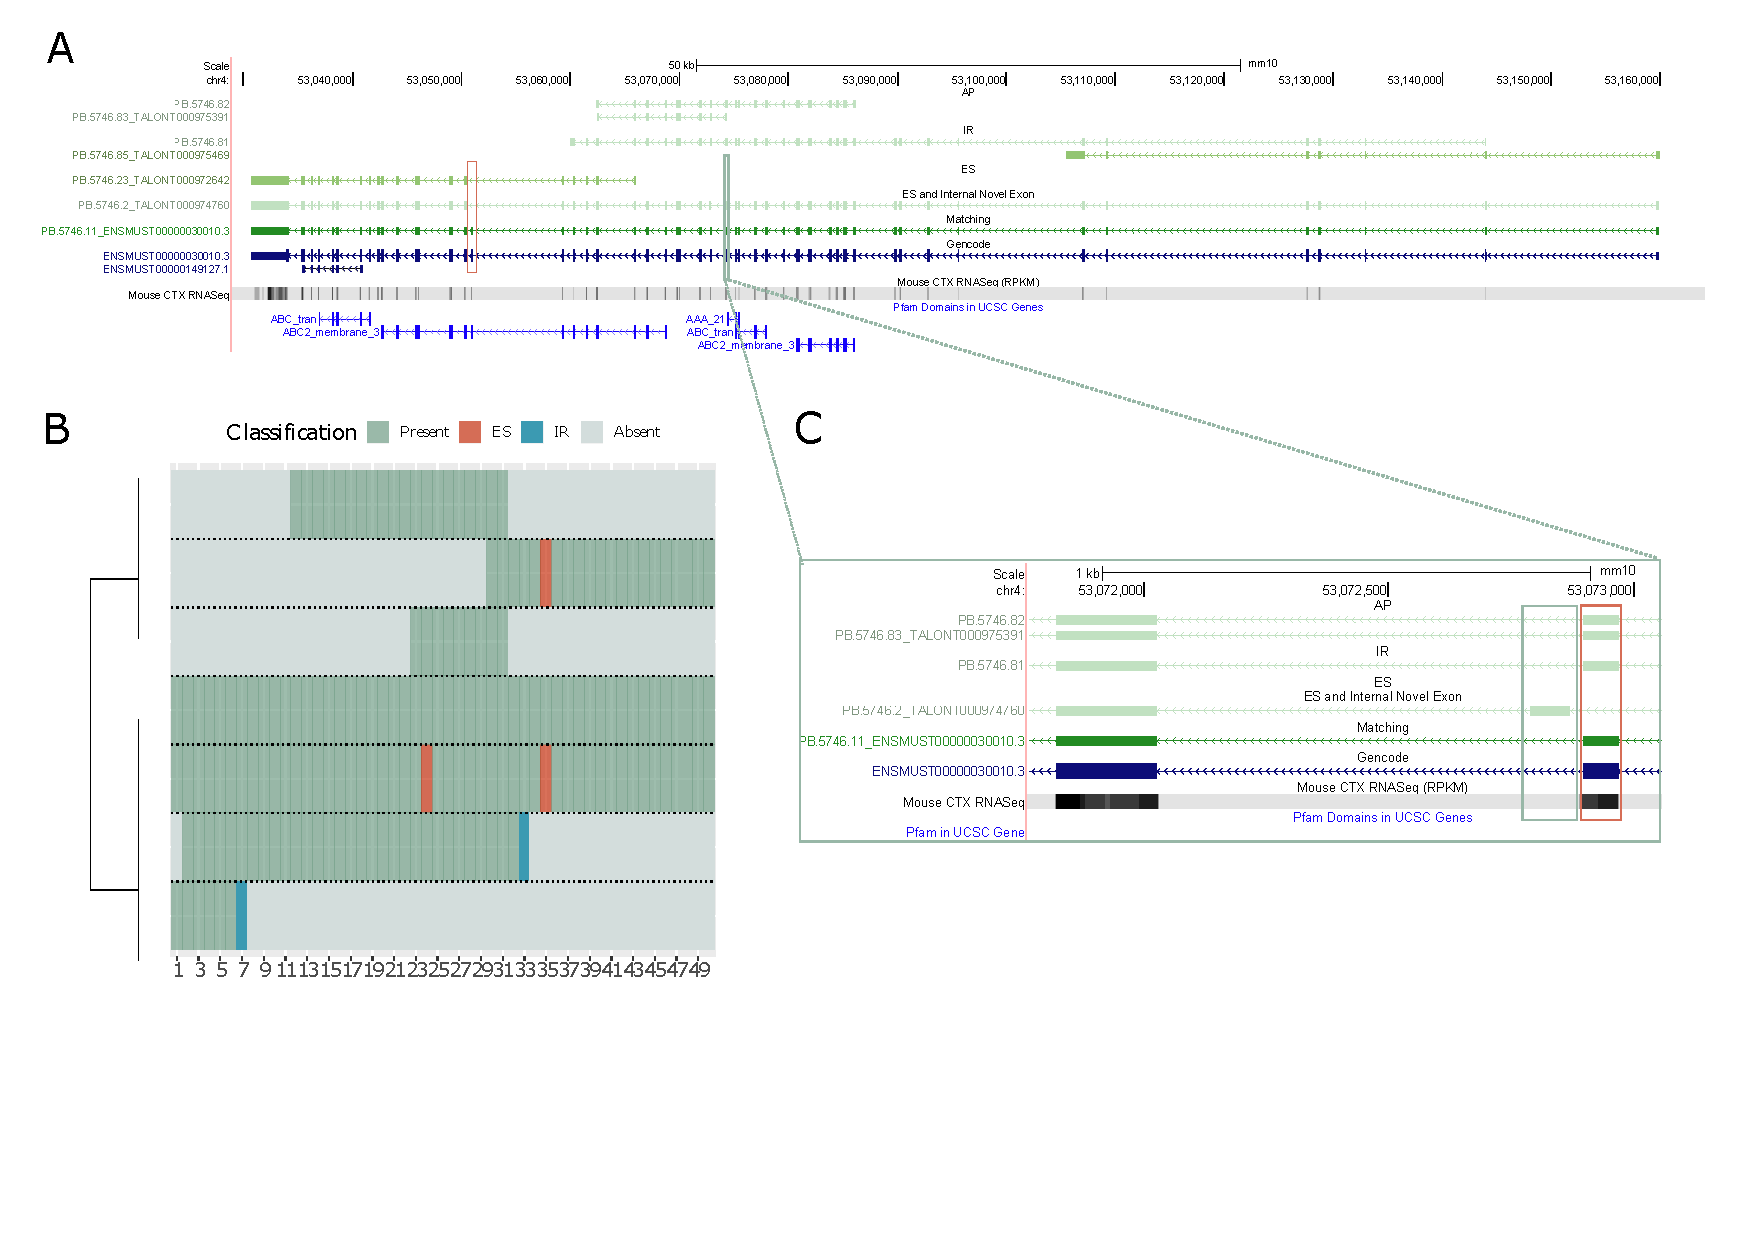
\includegraphics[page=1,trim={0 1cm 0 0},scale = 0.85]{Figures/TargetGenes_Annotation_Landscape.pdf}
		\end{center}
		\captionsetup{width=0.95\textwidth}
		\caption[RNA-Seq defined transcriptome]%
		{\textbf{}: }   
		\label{fig:abca1}
	\end{figure}
\end{landscape}

\newpage
\subsubsection{Trpa1}
From the panel of AD-associated genes enriched in the rTg4510 mouse cortex, \textit{Trpa1} - the ion channel receptor - was the least abundant and characterised with the fewest number of isoforms (n = 4) (\cref{fig:rhbdf2}\textbf{A}). Aside from detecting one of the two known canonical isoforms (Trpa1-201, ENSMUST00000041447.4), we further identified 2 novel isoforms that spanned the full-length of the known isoform and a short non-coding novel isoform (\cref{fig:rhbdf2}\textbf{A,B}). Blast analysis of the 2 novel isoforms and known isoform revealed that the exonic structure was generally conserved across the gene, with the exception of skipping of exon 20, varying lengths of the 5' and 3' UTR, and a 4-nucleotide addition at the end of exon 6 (\cref{fig:rhbdf2}\textbf{C}); RNA-Seq data from matched samples validate this 3' extension. 

ORF prediction of skipping of exon 20, which encodes for part of the ion channel domain, shortened but maintained the reading frame. However, strikingly, the most well-predicted ORF of the two novel isoforms was shifted significantly with initiation at a downstream AUG codon (\cref{fig:rhbdf2}\textbf{A}). Further examination of the ORF predicted using \textit{CPAT} revealed two alternative ORF initiated from the upstream AUG codon, but resulted in premature termination with an in-frame stop codon due to the addition of 4 nucleotides at exon 6. Conversely, the reading frame was intact for the known isoform.             

\begin{landscape}
	\begin{figure}[htp]
		\begin{center}
			\includegraphics[page=14,trim={0 1cm 0 0},scale = 0.85]{Figures/TargetGenes_Annotation_Landscape.pdf}
		\end{center}
		\captionsetup{width=0.95\textwidth}
		\caption[RNA-Seq defined transcriptome]%
		{\textbf{}: }   
		\label{fig:trpa1}
	\end{figure}
\end{landscape}

\newpage
\subsubsection{Rhbdf2}
The second least expressed gene within the panel of AD-associated target genes, \textit{Rhbdf2} was characterised with 5 isoforms and the least complex splicing pattern. Identifying two novel isoforms that spanned the length of the known detected canonical isoform (\cref{fig:rhbdf2}\textbf{A}), we detected exon skipping of exon 3 and exon 18 (\cref{fig:rhbdf2}\textbf{B}). While ORF prediction showed that all the isoforms generated a significantly shorter reading frame with usage of a downstream start codon, skipping of exon 18 resulted in a shorter terminal exon, which encoded for the rhomboid domain and is conserved in human (\cref{fig:rhbdf2}\textbf{A}). Similarly, the novel transcript with skipping of exon 3 had a shifted reading frame, however it was difficult to determine whether this was due to exon skipping or presence of an alternative first exon. Lastly, we detected a novel isoform that contained all the exons and was almost identical to the known isoform bar the deletion of 5 nucleotides from exon 7, which encodes for the protease domain. Strikingly, ORF prediction of this transcript revealed that this 3' truncation was accompanied with an even shorter reading frame (\cref{fig:rhbdf2}\textbf{C}).   

\begin{landscape}
	\begin{figure}[htp]
		\begin{center}
			\includegraphics[page=9,trim={0 1cm 0 0},scale = 0.85]{Figures/TargetGenes_Annotation_Landscape.pdf}
		\end{center}
		\captionsetup{width=0.95\textwidth}
		\caption[RNA-Seq defined transcriptome]%
		{\textbf{}: }   
		\label{fig:rhbdf2}
	\end{figure}
\end{landscape}

\newpage
\subsubsection{Ank1} 
From the panel of AD-associated target genes, \textit{Ank1} stood out for the domination of significantly shorter known canonical isoforms (\cref{fig:Ank1_track}\textbf{A}). While we did detect several longer known canonical isoforms (n = 4, 23.5\%, length = 6.5 - 8.2kb), the majority (n = 11, 64.7\%) were less than \textasciitilde 2kb long and spanned the last few exons. Furthermore, the two most-abundant isoforms annotated to \textit{Ank1} using both PacBio Iso-Seq and ONT were one of the short known isoforms (Ank1-208, ENSMUST00000121075.7) and the short non-coding isoform (Ank1-211, ENSMUST00000130311.1). %Although we are unable to rule out the technical limits of sequencing the longer transcripts, given that \textit{Ank1} is one of the longer genes from the panel of target genes,  

Aside from the length disparities among the isoforms detected, we found that the splicing pattern was generally conserved across the gene with consistent skipping of certain exons (\cref{fig:Ank1}\textbf{B}). Across all the long isoforms, exon 44 was skipped whereas exon 46 was skipped in half of the short isoforms (n = 4). While ORF prediction showed that skipping of the earlier exons shortened but maintained the reading frame, inclusion of exon 44 resulted in the inclusion of a stop codon and resulted in premature termination with predicted NMD. Conversely, isoforms that skipped exon 44 maintained the reading frame to the final exon and was not predicted for NMD  
(\cref{fig:Ank1_track}\textbf{B}).   

\begin{landscape}
	\begin{figure}[htp]
		\begin{center}
			\includegraphics[page=3,trim={0 1cm 0 0},scale = 0.85]{Figures/TargetGenes_Annotation_Landscape.pdf}
		\end{center}
		\captionsetup{width=0.95\textwidth}
		\caption[RNA-Seq defined transcriptome]%
		{\textbf{}: }   
		\label{fig:ank1}
	\end{figure}
\end{landscape}     

\newpage
\subsubsection{Cd33}
In total, we detected 41 isoforms associated with \textit{Cd33}, including 5 of the known isoforms (\cref{fig:cd33_track}). Reflecting the diversity of \textit{Cd33} known isoforms, the majority of isoforms detected were similarly short, lacked the first two upstream exons and also skipped exon 8 which was only present in the Cd33-201 known isoform (ENSMUST00000004728.11) (\cref{fig:Cd33}\textbf{A}, \cref{fig:cd33_track}). ORF predictions showed that skipping of this exon slightly reduced but maintained the reading frame (\cref{fig:cd33_track2}\textbf{A}). Conversely, 3'truncation of exon 4 (which encodes for the V-set domain) shifted the reading frame with the generation of a stop codon and subsequent usage of the downstream initiator codon in exon 2 (\cref{fig:cd33_track2}\textbf{A}).   

While the majority of isoforms were short, we detected a few novel, "full-length" isoforms that incorporated different features from the reference isoform (\cref{fig:cd33_track2}\textbf{B}); i.e. contained the upstream exons only present in the Cd33-202 known isoform (ENSMUST00000039861.6) while harbouring the longer 3'UTR present in the Cd33-203 known isoform (ENSMUST00000205503.1). Notably, we detected two very similar "full-length" isoforms that both contained a novel upstream exon between exons 1 and 2 (66bp, Chr7:43529866-43529932, \cref{fig:cd33_track2}\textbf{B}). However strikingly, due to similar 3' truncation of exon 4, ORF prediction of these two isoforms similarly revealed a shortened reading frame starting from exon 2 despite the presence of upstream exons.  

In contrast to exon skipping, we observed multiple intron retention events (IR) across the gene with over a third of isoforms (n = 14, 34.21\%) containing at least one IR event (\cref{fig:Cd33}\textbf{B}), and one isoform containing an intron retention event that spanned 4 exons (TALONT001237573, \cref{fig:cd33_track2}\textbf{C}). Further examination revealed that intron retention primarily occurred around exon 7 (\cref{fig:Cd33}\textbf{A}) and extended to the final two exons, exon 8 and 9, with varying lengths (\cref{fig:cd33_track2}\textbf{C}). ORF predictions showed that an extended intron retention at exon 7 revealed a stop codon resulting in a shortened reading frame, whereas an intact exon 7 resulted in a slightly longer reading frame.

\begin{landscape}
	\begin{figure}[htp]
		\begin{center}
			\includegraphics[page=4,trim={0 1cm 0 0},scale = 0.85]{Figures/TargetGenes_Annotation_Landscape.pdf}
		\end{center}
		\captionsetup{width=0.95\textwidth}
		\caption[RNA-Seq defined transcriptome]%
		{\textbf{}: }   
		\label{fig:cd33}
	\end{figure}
\end{landscape}    

\begin{landscape}
	\begin{figure}[htp]
		\begin{center}
			\includegraphics[page=5,trim={0 1cm 0 0},scale = 0.85]{Figures/TargetGenes_Annotation_Landscape.pdf}
		\end{center}
		\captionsetup{width=0.95\textwidth}
		\caption[RNA-Seq defined transcriptome]%
		{\textbf{}: }   
		\label{fig:cd33_orf}
	\end{figure}
\end{landscape}    

\subsubsection{Sorl1}
Although we detected 113 isoforms associated with \textit{Sorl1} - a gene which encodes for the endocytic receptor involved in APP trafficking - the splicing pattern was relatively simple with the internal exonic structure largely conserved and only a few isoforms exhibiting exon skipping and intron retention events (\cref{fig:sorl1}\textbf{A}, \cref{fig:sorl1_track1}). Strikingly, isoform diversity was primarily driven by usage of alternative promoter and termination usage while preserving the internal exonic structure (\cref{fig:sorl1_track2}\textbf{A}). Over 75\% (n = 88, 77.9\%) of the isoforms detected were characterised with a slightly different downstream first exon, which can be further broadly classified into three groups by presence of an alternative last exon at exons 37, 38 and 41 (\cref{fig:sorl1_track2}\textbf{B}). Furthermore, the alternative last exons do not fully match the exon of interest, resulting in enrichment of isoforms with A3' truncation of exon 37, 38, and 41 (\cref{fig:sorl1}\textbf{B}). Notably, exons 37 and 38 encode for Fibronectin type III domain, which is the largest protein domain of the SORL1 protein, and of which studies have previously identified rare AD-associated variants to be located within\cite{Verheijen2016}. ORF prediction of these isoforms with alternative promoter and terminator usage show shortened but otherwise intact reading frames with no prediction for NMD. 

\begin{landscape}
	\begin{figure}[htp]
		\begin{center}
			\includegraphics[page=10,trim={0 1cm 0 0},scale = 0.85]{Figures/TargetGenes_Annotation_Landscape.pdf}
		\end{center}
		\captionsetup{width=0.95\textwidth}
		\caption[RNA-Seq defined transcriptome]%
		{\textbf{}: }   
		\label{fig:sorl1}
	\end{figure}
\end{landscape}   

\newpage
\subsubsection{Vgf}
We detected 90 isoforms associated with \textit{Vgf}, despite it only containing 5 exons. Examination of this gene, which encodes for a neurosecretory protein that is cleaved into various peptides, remarkably suggested a relatively simple splicing pattern (\cref{fig:vgf}\textbf{A}): no detection of the first two upstream exons present in only one of the known isoform, the majority of isoforms skipped exon 5 and a few intron retention events were observed. However, further examination revealed complex variations of the final exon and 3'UTR (\cref{fig:vgf}\textbf{B})), as supported by matched RNA-Seq data (\cref{fig:vgf_track}). The vast majority of isoforms detected (n = 87, 96.7\%) were characterised with either an alternative 5' start sites (n = 35 isoforms, 38.9\%) or 3'end of the last exon (n = 4, 0.04\%), or with matched 5' and 3' end sites but skipping within the exon resulting in two enclosed exons (\cref{fig:vgf_track}). This phenomenon of skipping within the exon further extended beyond exon 6 in a few intron-retained isoforms. Given that isoforms exhibiting this "internal exon skipping" were detected in both PacBio Iso-Seq and ONT with stringent filtering, these are unlikely to be artefacts. 

ORF predictions of these isoforms showed that while this internal skipping phenomenon did not result in NMD, it generated significant variations of the reading frame particularly at the 3'end. Conversely, isoforms with alternative 5' start site of the last exon were predicted as either non-coding or missing an ORF.

\begin{landscape}
	\begin{figure}[htp]
		\begin{center}
			\includegraphics[page=15,trim={0 1cm 0 0},scale = 0.85]{Figures/TargetGenes_Annotation_Landscape.pdf}
		\end{center}
		\captionsetup{width=0.95\textwidth}
		\caption[RNA-Seq defined transcriptome]%
		{\textbf{}: }   
		\label{fig:vgf}
	\end{figure}
\end{landscape} 

\newpage
\subsubsection{Fyn}
Known to directly phosphorylate and interact with tau, \textit{Fyn} encodes for a tyrosine kinase that is associated with several known isoforms that primarily differ in the first exon from usage of alternative promoter. Detecting in total 50 isoforms, we found these first exons to be mutually exclusive with either isoforms containing exon 1, 2 or 4 (\cref{fig:fyn}). In contrast, we did not detect the shorter isoforms with the most downstream alternative promoter at exon 5 or 6. However, we did detect a significant number of isoforms (n = XX) that contained novel first exons at 3 distinct positions; between exons 2 and 3, 4 and 5, and even further downstream at exon 8. Strikingly, the novel exon between exons 4 and 5 was found in isoforms with alternative 4 exon, highlighting the complexity of alternative promoter usage in \textit{Fyn}. Of note, ORF predictions of these isoforms with novel exons did not change the reading frame, and similarly exon skipping shortened but otherwise maintained reading frame.  

In contrast to the complexity at the 5'end of the gene, the exonic structure downstream of exon 7 was relatively conserved across the majority of isoforms. Particularly exons between exon 7 and 12, which encode for the SH3 domain known to interact with tau, were present across all the isoforms (\cref{fig:fyn_track}). Conversely, exons 13 and 14,  which encode for the protein kinase domain, were found to be mutually exclusive with the majority of detected isoforms containing exon 13 (n = 36) and skipping exon 14 (\cref{fig:fyn_track}). Finally, we noted a complete absence of exon 16, which originated from an alternative first exon of the shortest known isoform. 

\begin{landscape}
	\begin{figure}[htp]
		\begin{center}
			\includegraphics[page=7,trim={0 1cm 0 0},scale = 0.85]{Figures/TargetGenes_Annotation_Landscape.pdf}
		\end{center}
		\captionsetup{width=0.95\textwidth}
		\caption[RNA-Seq defined transcriptome]%
		{\textbf{}: }   
		\label{fig:fyn}
	\end{figure}
\end{landscape} 

\newpage
\subsubsection{Picalm}
In total, we detected 144 isoforms associated with \textit{Picalm}, a gene that encodes for an adaptor protein that is involved with APP trafficking and endocytosis. Of these 144 isoforms, we identified all the known isoforms, including the mono-exonic isoforms, bar the non-coding isoform Picalm-208	 (ENSMUST00000207949.1). Approximately a fifth of the isoforms (n = 31, 21.5\%) detected spanned the "full-length" of the gene from exon 1 to 21, while the remaining isoforms were significantly shorter with alternative first exon and promoter usage from every exon. Of note, we identified a novel isoform that contained a novel first exon 59kb upstream of known exon 1 and was detected using both PacBio Iso-Seq and ONT (PB.7635.2-TALONT001254093).

While exon skipping was observed consistently at exons 13, 18, and 21, which do not encode for any Pfam domains, the internal exonic structure was broadly conserved. ORF predictions showed that skipping of such exons shortened but maintained the reading frame. \textit{Picalm} isoform diversity was subsequently driven by usage of alternative first exon and promoter. Such shorter isoforms are unlikely to be artefacts given that a few of the known isoforms display similar feature (i.e partial subset of the longer "full-length" isoforms), a significant number (n = 66, 60\%) were detected using both long-read sequencing approaches, and after performing stringent filtering. 

%However, the vast majority of coding isoforms were predicted to undergo nonsense mediated decay (n = 115, 98.3\%) including the known reference isoforms. Further examination revealed that while the reading frame varied at the 5'end from alternative first exon usage, all the reading frames 

\begin{landscape}
	\begin{figure}[htp]
		\begin{center}
			\includegraphics[page=8,trim={0 1cm 0 0},scale = 0.85]{Figures/TargetGenes_Annotation_Landscape.pdf}
		\end{center}
		\captionsetup{width=0.95\textwidth}
		\caption[RNA-Seq defined transcriptome]%
		{\textbf{}: }   
		\label{fig:picalm}
	\end{figure}
\end{landscape} 

\subsubsection{Tardbp}
\textit{Tardbp} encodes for TDP-43, aggregates of which are frequently observed in multiple neurodegenerative diseases including ALS and FTD. Although not the primary hallmark of AD, up to 75\% of AD patients are also presented with TDP-43 aggregates. Despite only containing 10 exons, \textit{Tardbp} is one of the most complex gene from the targeted panel of AD-associated genes; various isoforms contain exon overlap at multiple regions at the 3'end from exon 6 onwards. The complexity is reflective of the "internal exon skipping" phenomenon observed in the final exon of \textit{Vgf}, with added complexity from additional usage of alternative termination and 3'sites of the last exon. This complexity was also captured in our targeted dataset with detection of known isoforms either with matching or slight wobble splice sites. We also detected novel isoforms with a combination of exons from different known isoforms; e.g. a novel isoform (PB.6120.170) that contained all the exons from ENSMUST00000190287.1 and the upstream first three exons from the longer "full-length" known isoforms. 

Despite the complexity of the 3'end of \textit{Tardbp}, we observed a relatively consistent splicing pattern with multiple intron retention events, particularly between exons 6 and 7. A XX of isoforms were also identified with an alternative last exon accompanied with terminal intron retention at exons 7 and 8. Conversely, exons 2 to 4, which encode for RNA recognition motif domain were present and structurally preserved in the majority of isoforms.  

\begin{landscape}
	\begin{figure}[htp]
		\begin{center}
			\includegraphics[page=11,trim={0 1cm 0 0},scale = 0.85]{Figures/TargetGenes_Annotation_Landscape.pdf}
		\end{center}
		\captionsetup{width=0.95\textwidth}
		\caption[RNA-Seq defined transcriptome]%
		{\textbf{}: }   
		\label{fig:tardbp}
	\end{figure}
\end{landscape} 

\newpage
\subsubsection{Mapt}
The aggregation of tau, which is encoded by \textit{Mapt}, into neurofibrillary tangles is one of the two key hallmarks of AD. To study splicing changes associated with progression of tau pathology, we used rTg4510 mouse model which harbours the human tau transgene, Mapt\textsuperscript{P301L}. As previously shown, human-specific \textit{MAPT} transcripts were only detected in TG mice and were removed for downstream analysis, retaining only mouse-specific \textit{Mapt} transcripts. 

In total, we detected 140 isoforms associated with \textit{Mapt}, including 7 of the known isoforms. Upon further examination of these isoforms, one of the most striking splicing feature observed was the number of consistent exon skipping events that alternated across the gene. The majority of isoforms were characterised with at least one exon skipping event (n = 115, 82.1\%) with most isoforms skipping 3 exons or more (n = 98); notably, we detected an isoform with extensive skipping of 12 exons. Despite the widespread occurrence of exon skipping, we found that the splicing pattern was conserved across the isoforms with skipping of alternative exons; i.e. exons 4, 6, 8, 10 and 13. In contrast, exons 2, 7, 11, 12 and 14, which were present in all the known isoforms (i.e. constitutive) were also present in all the isoforms that spanned the "full-length" of the gene. 

Detected in both PacBio Iso-Seq and ONT, we identified a number of isoforms with novel first exons located between exon 1 and 2 (n = 16, 11.4\%), which were broadly clustered into five groups and indicated alternative promoter usage. Notably, some of these novel exons were also contained within the other isoforms. ORF prediction of these isoforms showed that usage of these alternative first exons shortened but maintained the reading frame. 

Finally, we detected some significantly shorter isoforms that were distinguished by the presence of a intron-retained first exon. These broadly appeared between exons 9 and 11 which encode for the tubulin-binding repeat domain. 


\begin{figure}[htp]
	\begin{center}
		\includegraphics[page=5,trim={0 1cm 0 0},scale = 0.85]{Figures/TargetGenes_Annotation_Portrait.pdf}
	\end{center}
	\captionsetup{width=0.95\textwidth}
	\caption[RNA-Seq defined transcriptome]%
	{\textbf{}: }   
	\label{fig:mapt}
\end{figure}

\newpage
\subsubsection{Fus}
Identified as a causative gene for amyotrophic lateral sclerosis (ALS) and FTD, \textit{Fus} has become the characteristic pathological hallmark for neuronal aggregation in the subset of sporadic FTD cases that lack the more established inclusion markers of TDP-43 and tau\cite{Seelaar2010}. Despite only containing 15 exons, \textit{Fus} is a complex gene; multiple isoforms with varying lengths and exon inclusion are generated with only a quarter of the known isoforms (n = 4, 25\%) spanning the full-length of the gene. In total, we detected a total of 236 isoforms annotated to \textit{Fus}, the majority of which were "full-length" (n = 154, 58.6\%). Consequently in contrast to the known \textit{Fus} isoform landscape in the mouse genome, we found the \textit{Fus} splicing pattern relatively simpler in our dataset. A quarter (n = 53, 25.7\%) of the isoforms detected were largely analogous to the "full-length" isoform in preserving the exonic structure, differing by minor variations ("wobble") at the splice site. 

Nonetheless, we detected widespread occurrence of exon skipping and intron retention events that were not observed in the reference genome. Over 40\% of isoforms (n = 103, 43.6\%) were characterised with at least one exon skipping event, with exon 8 exclusion observed in almost half of the these isoforms (n = 50 isoforms with exon 8 skipped, n = 48.5\%). Around the same region, we also detected a number of isoforms with intron retention events spanning across exons 6 and 7, which are also identified in the novel isoforms. However notably, we noted an intron-retained isoform than incorporated one of the known mono-exonic isoforms, resulting in an intron retained region spanning exons 10-12 which encode the RNA recognition motif (RRM) domain. Finally, we detected a number of intron retention events at the 3'end of the gene between exons 12 and 14, which encode zinc-finger-containing RGG-Znf-RGG domain (zF-RanBP). As an RNA-binding protein and a subunit of the heterogeneous nuclear ribonucleoprotein complex (hnRNP) complex involved in splicing, FUS recognition of RNA is mediated by both the RRM and zF-RanBP domains\cite{Wang2015c}. 

\begin{figure}[htp]
	\begin{center}
		\includegraphics[page=4,trim={0 1cm 0 0},scale = 0.85]{Figures/TargetGenes_Annotation_Portrait.pdf}
	\end{center}
	\captionsetup{width=0.95\textwidth}
	\caption[RNA-Seq defined transcriptome]%
	{\textbf{}: }   
	\label{fig:fus}
\end{figure}

\newpage
\subsubsection{Bin1}
\textit{Bin1} has been well implicated in AD pathology through identification of multiple AD-associated SNPs from GWAS studies, and recent studies on human post-mortem AD brains have shed light on the function and differential expression of its associated isoforms\cite{Taga2020}. Drawing parallels to the human-equivalent \textit{Bin1} isoforms\cite{Taga2020}, we observed extensive exon skipping within certain parts of the gene; the majority of isoforms (n = 290 isoforms, 78.8\%) were characterised with at least one exon skipping event. The first 10 exons encoding the N-BAR domain, which is involved in membrane curvature, were conserved and included in the "full-length" isoforms. Conversely inclusion of exons 14-16, which encode the CLAP domain involved in endocytosis, was highly variable among isoforms (Exon 14 skipping: 104 isoforms, Exon 15 skipping: 174 isoforms, Exon 16 skipping: 249 isoforms). However, intron retention events (n = 48 events, 25 isoforms) were also notably enriched within this region. Aside from detecting long isoforms spanning the full-length of the gene, we also detected shorter isoforms with exclusion of the initial exons encoding the N-BAR domain but inclusion of the terminal exons encoding the Src homology 3 (SH3) domains. Among these, a number of isoforms (n = 19, 13.2\%) were relatively similar in length and exonic structure to Bin1-204 (ENSMUST00000234373.1) with a long alternative first exon encoding the CLAP domain.  

\begin{figure}[htp]
	\begin{center}
		\includegraphics[page=3,trim={0 1cm 0 0},scale = 0.85]{Figures/TargetGenes_Annotation_Portrait.pdf}
	\end{center}
	\captionsetup{width=0.95\textwidth}
	\caption[RNA-Seq defined transcriptome]%
	{\textbf{}: }   
	\label{fig:bin1}
\end{figure}

\newpage
\subsubsection{App}
\textit{App}, encoding for amyloid precursor protein, is one of the most commonly involved gene for AD with \textasciitilde30 causative mutations described. Detecting a total of 466 isoforms annotated to \textit{App}, we observed varying isoform lengths with less than half of the isoforms (n = 183, 39.9\%) containing exon 1 and spanning the full length of the gene. While a number of isoforms were structurally analogous to the two known shorter isoforms - App-205 (ENSMUST00000227654.1) and App-210 (ENSMUST00000228375.1) - we detected a significant number that started with a novel alternative first exon between exons 3 and 5, which encode the APP heparin binding domain. Nonetheless, the variation typically resided within the 5' end of the gene with the vast majority of isoforms (n = 428, 91.8\%) containing the terminal exon, which encode the cleaved beta amyloid peptide. 

Despite this length variation, we observed a consistent splicing pattern with exon skipping (n = 406 isoforms, 87.1\%) enriched in two regions of the gene: across exon 7 (n = 289 isoforms) and exon 8 (n = 304 isoforms), which encode the Kunitz-type protease inhibitor (KPI), and exons 14 (n = 392 isoforms) and 15 (n = 390 isoforms), which were alternative last exons present in only two of the known \textit{APP} isoforms (App-208, ENSMUST00000227753.1 and App-209, ENSMUST00000227990.1). Previous studies to characterise \textit{App} isoforms have reported exon skipping of the KPI domain with conflicting results reported for the differential expression of KPI-containing isoforms in AD post-mortem brains. Despite enrichment of exon skipping within these two regions, exon skipping was widespread across the gene with majority of isoforms detecting characterised with 4 or more skipping events (n = 291 isoforms, 71.7\% of ES-isoforms). This included skipping of exons 18 and 19, which encode the beta-amyloid precursor protein C-terminus that is strongly implicated in AD and are often skipped together.   

\begin{figure}[htp]
	\begin{center}
		\includegraphics[page=2,trim={0 1cm 0 0},scale = 0.85]{Figures/TargetGenes_Annotation_Portrait.pdf}
	\end{center}
	\captionsetup{width=0.95\textwidth}
	\caption[RNA-Seq defined transcriptome]%
	{\textbf{}: }   
	\label{fig:app}
\end{figure}

\newpage
\subsubsection{Ptk2b}
\textit{Ptk2b}, which encodes for protein tyrosine kinase 2 (Pyk2), was one of the few genes for which altered splicing was reported to be a direct mechanism for the effects of AD-associated variants identified from human GWAS studies\cite{Raj2018}. Although increased intron retention was reported from a AD TWAS study\cite{Raj2018}, we observed that the \textit{Ptk2b} isoform landscape (n = 563 isoforms) in our dataset was dominated by varying isoform lengths with usage of alternative first exon and exon skipping, particularly exon 27 (n = 296, 52.5\%). ORF predictions showed that skipping of this 24bp exon, which was included in all the known isoforms (i.e. "constitutive"), shortened but maintained the reading frame. Conversely, intron retention was only evident in a few isoforms (n = 6, 1.1\%, detected using both PacBio Iso-Seq and ONT nanopore sequencing), which were analogous in exonic structure to the known shorter isoform (Ptk2b-205, ENSMUST00000136216.7) spanning the 3'end of the gene. 

Drawing parallels to the human-equivalent \textit{PTK2B}, the mouse \textit{Pt2kb} gene similarly encompasses several well-defined structural domains including the N-terminal FERM domain, a central tyrosine kinase domain, and a C-terminal focal adhesion targeting domain (FAT)\cite{DePins2021}. Deeper characterisation of \textit{Pt2kb}-annotated isoforms in our dataset revealed isoforms with varying lengths from 5'truncation of the gene; i.e. the first exon starts downstream and contain exons encoding the kinase and FAT domain but lack the N-terminal FERM domain. Given that we performed stringent processing and filtering, it is unlikely that these isoforms are a by-product of RNA degradation, particularly given a number of these isoforms were detected by both long-read sequencing technologies and half of the known \textit{Ptk2b} isoforms exhibit a similar exonic structure. Previous studies have also identified similar isoforms that lack the FERM and kinase domain, and is predicted to be transcribed from an alternative promoter as an endogenous regulator of Pyk2 activity\cite{DePins2021}. Finally, we noticed that while the splice sites were largely conserved across the gene, exon 26 - the neighbouring exon to exon 27 which was skipped in half of the isoforms, was characterised with extensive A3' extension (i.e. matched 5' splice site but varying 3' splice site to the known isoform). 

\begin{figure}[htp]
	\begin{center}
		\includegraphics[page=6,trim={0 1cm 0 0},scale = 0.85]{Figures/TargetGenes_Annotation_Portrait.pdf}
	\end{center}
	\captionsetup{width=0.95\textwidth}
	\caption[RNA-Seq defined transcriptome]%
	{\textbf{}: }   
	\label{fig:ptk2b}
\end{figure}

\newpage
\subsubsection{Snca}
\textit{Snca} encodes for $\alpha$-synuclein, which is known to abnormally aggregate in patients with PD, DLB and AD as a defining hallmark of Lewy body pathology. Despite only containing 7 exons, \textit{Snca} was the third most "isoformic" gene from the targeted panel with 622 isoforms detected. Deeper characterisation revealed that exon skipping, alternative 5' and 3' start sites largely contributed to the isoform diversity. Over 75\% of isoforms (n  = 483, 77.7\%) were identified with at least one exon skipping event. Exon 4 and 5 were skipped the most (exon 4: n = 249 isoforms; exon 5: n = 206 isoforms), despite being present across all the reference isoforms including the two known shorter isoforms (i.e constitutive). Aside from exon skipping, extensive usage of alternative 5' and 3' sites, particularly A5' truncation, was observed across all the exons with the exception of exon 4. Of note, we detected 84 isoforms which contained all the exons and primarily differed by alternative 5' and 3' sites. 
%Approximately two-thirds of isoforms detected were non protein-coding (n = 402, 64\%). 

\begin{figure}[htp]
	\begin{center}
		\includegraphics[page=7,trim={0 1cm 0 0},scale = 0.85]{Figures/TargetGenes_Annotation_Portrait.pdf}
	\end{center}
	\captionsetup{width=0.95\textwidth}
	\caption[RNA-Seq defined transcriptome]%
	{\textbf{}: }   
	\label{fig:snca}
\end{figure}

\subsubsection{Clu}
In line with previous findings from human studies, we identified multiple isoforms (n = 733) annotated to \textit{Clu} in the mouse cortex. Although \textit{Clu}'s known isoform landscape was dominated by the presence of alternative first exons (n = 6 alternative first exons across 9 known isoforms), the majority of detected isoforms (n = 402, 55\%) originated from the first upstream exon and spanned the full-length of the gene. However, we did identify a handful of novel isoforms (n = 12, 1.6\%) with various alternative first exon, indicating the importance of alternative promoter usage as a transcriptional mechanism of \textit{Clu} expression.

Deeper characterisation revealed that \textit{Clu} isoform diversity in our dataset was driven primarily by extensive usage of alternative 5' and 3' splice sites, and exon skipping and intron retention events enriched in certain parts of the gene. While we detected some degree of exon skipping across all the exons, exon 9 (n = 143 isoforms, 19.5\%), exon 10 (n = 129 isoforms, 17.6\%) and exon 11 (n = 165 isoforms, 22.5\%) were notably more skipped. Adding to the complexity of splicing in \textit{Clu}, these ES-annotated-isoforms were further characterised with alternative 5' and 3' splice sites in the exons included; Exon 10 was identified as one of the most skipped and most varied exon with alternative splice sites. In contrast, intron retention events (n = 217 events) predominantly occurred at the 5'end of the gene between exons 7 and 8. Notably, we identified a number of isoforms with intron retention spanning across exon 7 and upstream known alternative first exons; 42 isoforms with IR spanning across exon 7 and alternative first exon from Clu-206 (ENSMUST00000144619.1) and 4 isoforms with IR spanned across alternative first exon from Clu-203 (ENSMUST00000128539.7). 

\begin{landscape}
	\begin{figure}[htp]
		\begin{center}
			\includegraphics[page=6,trim={0 1cm 0 0},scale = 0.85]{Figures/TargetGenes_Annotation_Landscape.pdf}
		\end{center}
		\captionsetup{width=0.95\textwidth}
		\caption[RNA-Seq defined transcriptome]%
		{\textbf{}: }   
		\label{fig:clu}
	\end{figure}
\end{landscape}

\newpage
\subsubsection{Apoe}
Despite only containing 5 exons, \textit{Apoe} - the strongest risk factor for AD - was annotated with the highest number of isoforms (n = 2,006). While the majority of isoforms contained all 5 exons (n = X), a deeper examination of \textit{Apoe} revealed complex variations of the final exon and 3'UTR, 
supported by RNA-Seq data from matched samples. Drawing parallels to \textit{Vgf} and akin to one of the known isoforms of \textit{Apoe} (ENSMUST00000167646.8), the vast majority of isoforms detected were characterised with matched A5' and 3' end sites of exon 6 but skipping within the exon, resulting in two enclosed exons. As the primary contributor of isoform diversity in \textit{Apoe}, we also further detected a number of short isoforms that only contained exon 6 with evidence of "internal exon skipping". 

In contrast to exon 6, the other exons were relatively conserved with significantly fewer variation of alternative 5' and 3' splice sites. Furthermore, despite the widespread isoform diversity identified for \textit{Apoe}, we only detected 4 isoforms that contained the known alternative first exon present in two of the known isoforms (ENSMUST00000172983.7). Notably, one of them (TALONT00166063) contained both the first exon and an alternative first exon, indicating that these exons are not mutually exclusive and further highlight the over-simplicity of the reference genome. 

Aside from extensive usage of alternative 5' and 3' splice site, we also detected relatively low occurrence of exon skipping (n = 125 isoforms (0.06\%), XX events) and intron retention (n = 4 isoforms, n = XX events ). Exon 5 was found to be skipped the most (n = 89, 71.2\% of isoforms with ES), followed by exon 4 (n = 61 isoforms, 48.8\%). 

\begin{figure}[htp]
	\begin{center}
		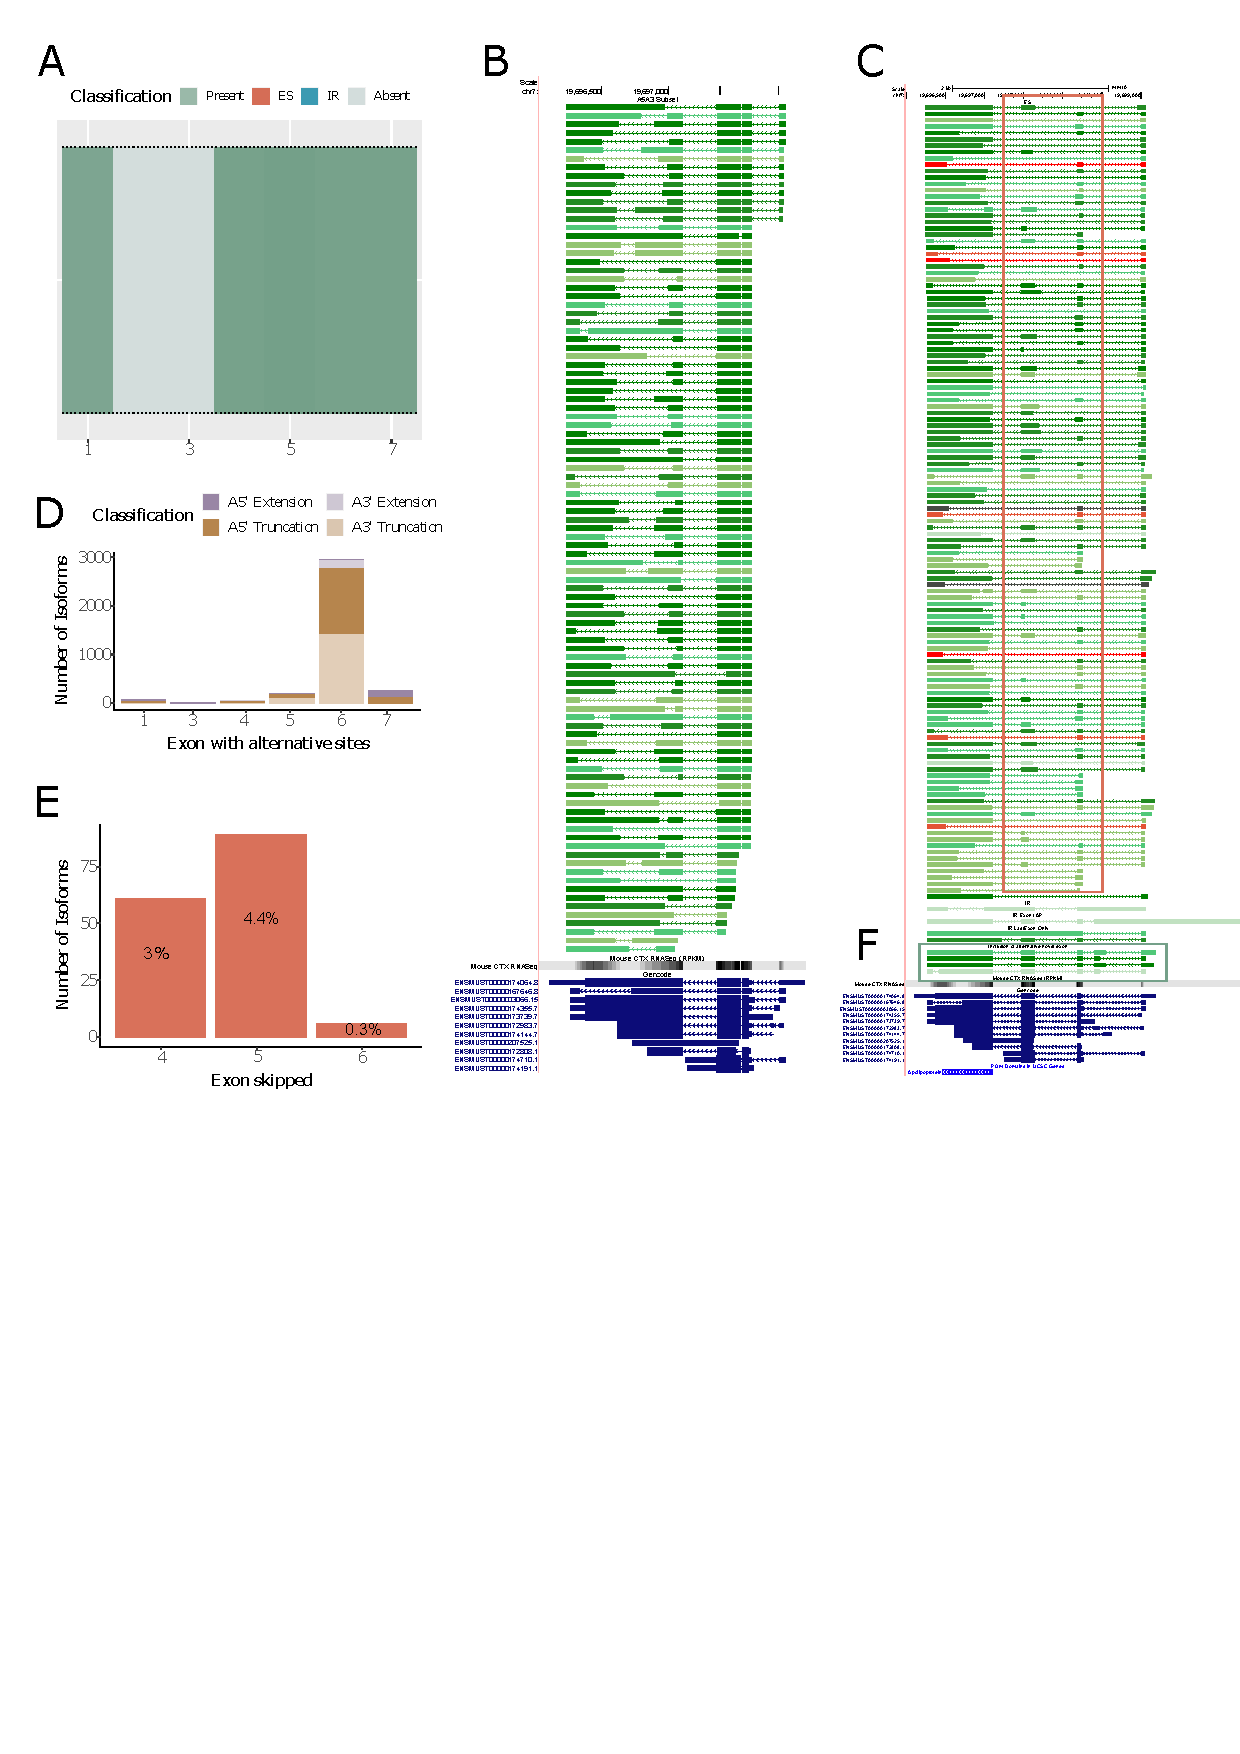
\includegraphics[page=1,trim={0 1cm 0 0},scale = 0.85]{Figures/TargetGenes_Annotation_Portrait.pdf}
	\end{center}
	\captionsetup{width=0.95\textwidth}
	\caption[RNA-Seq defined transcriptome]%
	{\textbf{}: }   
	\label{fig:apoe}
\end{figure}

\newpage
\subsection{Improved sensitivity from targeted sequencing detects upregulation of AD-associated genes in rTg4510 TG mice}
Despite the success of capturing full-length transcripts with long-read sequencing of the global transcriptome, we have shown that this approach falls short of sufficiently covering the more-lowly abundant genes and isoforms (\cref{ch6: wholevstargeted}). In contrast, target enrichment with CaptureSeq achieved deep sequencing of AD-associated genes, revealing unprecedented diversity of alternatively-spliced isoforms numbering in the hundreds (\cref{ch6: target_gene_annotation}). We suspected that this deep sequencing coverage would further allow accurate quantification of gene and isoform expression using normalised full-length read counts (\cref{fig:isoform_quant_strategy}\textbf{C}), forgoing the need of short-read RNA-Seq data (\cref{fig:isoform_quant_strategy}\textbf{B}). Subsequently, we sought to characterise transcriptional changes of these well known AD-associated genes between rTg4510 WT and TG mice by identifying changes in gene and isoform expression and usage.

Using targeted Iso-Seq reads for annotation and expression, we identified three genes that were upregulated with progressive tau pathology in rTg4510 TG mice: \textit{Trem2} (log\textsubscript{2} fold change (FC) = 2.26, P = 2.45 x 10 \textsuperscript{-16}, R\textsuperscript{2} = 0.788), \textit{Cd33} (log\textsubscript{2}FC = 1.79, P = 4.5 x 10 \textsuperscript{-9}, R\textsuperscript{2} = 0.588) and \textit{Rhbdf2} (log\textsubscript{2}FC = 1.39, P = 3.06 x 10 \textsuperscript{-6}, R\textsuperscript{2} = 0.5). Upregulation of these genes were also observed using normalised ONT read counts, and was significantly more robust due to the greater sequencing depth achieved with ONT nanopore sequencing (\textit{Trem2}: log\textsubscript{2} fold change (FC) = 2.47, P = 1.91 x 10 \textsuperscript{-40}, R\textsuperscript{2} = 0.938); \textit{Cd33}: log\textsubscript{2}FC = 2.25, P = 2.97 x 10 \textsuperscript{-20}, R\textsuperscript{2} = 0.823; \textit{Rhbdf2}: log\textsubscript{2}FC = 1.31, P = 1.36 x 10\textsuperscript{-6}, R\textsuperscript{2} = 0.564). Consequently, we detected a significant increase in \textit{Apoe} (log\textsubscript{2}FC = 1.44, P = 1.45 x 10\textsuperscript{-8},  R\textsuperscript{2} = 0.76), \textit{Clu} (log\textsubscript{2}FC = 1.36, P = 1.39 x 10\textsuperscript{-16}, R\textsuperscript{2} = 0.80) and \textit{Abca1} (log\textsubscript{2}FC = 1.56, P = 5.66 x 10\textsuperscript{-5}, R\textsuperscript{2} = 0.7) gene expression using normalised ONT but not Iso-Seq FL read counts. This is in line with a previous RNA-Seq study that reported upregulation of \textit{Trem2} and \textit{Apoe} in isolated-microglia from rTg4510 mice\cite{Sobue2021}. Notably, these gene expression changes were recapitulated using normalised RNA-Seq reads aligned to the whole transcriptome Iso-Seq dataset, but not from normalised Iso-Seq read counts from the whole transcriptome profiling, as further evidence of the greater sensitivity of targeted sequencing. 

Given the improved sensitivity of targeted sequencing and the extensive mapping of isoform landscape of AD-associated genes, we next sought to identify changes in transcript expression between rTg4510 TG and WT mice. In total, we detected 553 differentially expressed transcripts using normalised ONT reads counts, the majority (n = 485, 87.7\%) of which were associated with progressive tau pathology. Among these, 448 transcripts (81\%) were novel and \textit{Clu} was annotated with the most differentially expressed transcripts (n = 151, 31.1\%); no differential transcript expression was detected for \textit{Ank1, Tardbp} and \textit{Trpa1}. Despite this unprecedented detection of novel transcripts whose expression changed with increased tau pathology, we found that the majority (n = 366, 75.4\%) of these isoforms were lowly-expressed ($<$20 normalised FL read counts) and accounted less than 5\% of the respective isoform fraction. Further examination revealed that the isoform landscape across the 20 AD-associated genes were characterised by a few dominant isoforms. This corroborates with findings from the largest database genome-wide, quantitative profiles of AS events to date, reporting that more than 18\% of genes simultaneously express multiple major isoforms\cite{Tapial2017}. 

A reflection of the relatively lower sequencing depth of the Iso-Seq targeted dataset, we only detected 16 differentially expressed transcripts using Iso-Seq normalised read counts. Comparison of the ONT and Iso-Seq targeted dataset revealed 6 that were commonly identified as differentially expressed. Among these, the top ranked differentially expressed transcript was a known isoform (Trem2-201, ENSMUST00000024791.14) annotated to \textit{Trem2}. Expression of this known isoform significantly dominated that of the novel isoforms, and was strongly upregulated with progressive tau pathology; this was evident in both ONT and Iso-Seq targeted dataset. Drawing parallels to \textit{Gfap} and \textit{C4b}, upregulation of Trem2-201 mirrored that of \textit{Trem2} gene expression, indicating that increased \textit{Trem2} gene expression in aged rTg4510 TG mice was primarily driven by one dominant isoform. Despite this upregulation of Trem2-201, we found that there was no change in isoform usage across genotype or with age; Trem2-201 occupied over 75\% of the isoform proportion in rTg4510 irrespective of genotype and age. The remaining isoform proportions were equally divided into the two other known isoforms - Trem2-202 (ENSMUST00000113237.3) and Trem2-203 (ENSMUST00000113237.3) - and all of the other novel isoforms combined. These findings suggest that the drastic upregulation of the dominant isoform (Trem2-201) in aged rTg4510 TG mice was accompanied with an increased expression of all the other minor isoforms by the same magnitude, resulting in a consistent isoform proportion. Hierarchical clustering of individual mouse samples based on \textit{Trem2} isoform expression level was further found to robustly discriminate between TG and WT groups and by age, as evidence of the global increase of \textit{Trem2}-associated transcript expression with progressive tau pathology.  

Aside from \textit{Trem2}, we identified changes in expression of the known isoform annotated to \textit{Cd33} and \textit{Bin1} with accumulation of the tau pathology in rTg4510 TG mice. Using normalised ONT read counts, we noted a drastic increase in gene expression of \textit{Cd33} and its known isoform, Cd33-203 (ENSMUST00000205503.1) in aged rTg4510 TG mice. However, unlike \textit{Trem2}, the \textit{Cd33} isoform landscape was relatively more complex, suggesting that increased \textit{Cd33} gene expression is not solely driven by one isoform. Several novel isoforms were found to be abundantly expressed, occupying \textasciitilde50\% of \textit{Cd33} isoform proportion. Among these, two isoforms (TALONT001237522, TALONT001237572) were significantly upregulated with progressive tau pathology (TALONT001237572: log\textsubscript{2} FC = 2.65, P = 2.37 x 10\textsuperscript{-14}, R\textsuperscript{2} = 0.79, TALONT001237522: log\textsubscript{2} FC = 1.91, P = 7.62 x 10\textsuperscript{-25}, R\textsuperscript{2} = 0.90). Both isoforms differed from the known isoform by an alternative last exon characterised with intron retention of exons 7 and 8. Finally, we observed a notable change in isoform usage between rTg4510 TG and WT mice aged 8 months with upregulation of Cd33-203 coupled with downregulation of a novel mono-exonic isoform (TALONT001237520, P = 2.38 x 10\textsuperscript{-5}, R\textsuperscript{2} = 0.50) that spanned the 3'UTR. 

  

  


 
\begin{landscape}
	\begin{figure}[htp]
		\begin{center}
			\includegraphics[page=19,trim={0 0.5cm 0 1.5cm},scale =0.85]{Figures/TargetGene_DifferentialAnalysis.pdf}
		\end{center}
		\captionsetup{width=1.5\textwidth}
		\caption[Differential Isoform Expression: Changes in transcript expression of isoforms associated with \textit{Trem2}]%
		{\textbf{Significant upregulation of dominant known isoform of \textit{Trem2} with progressive tau pathology}: \textit{Caption continues on the following page.}}   
		\label{fig:trem2_diff_analysis}
	\end{figure}
\begin{figure}[p]
	\captionsetup{width=1.5\textwidth}
	\contcaption{\textbf{(A)} }%
\end{figure}
\end{landscape}

\begin{landscape}
	\begin{figure}[htp]
		\begin{center}
			\includegraphics[page=7,trim={0 0.5cm 0 1.5cm},scale =0.85]{Figures/TargetGene_DifferentialAnalysis.pdf}
		\end{center}
		\captionsetup{width=1.5\textwidth}
		\caption[Differential Isoform Expression: Changes in transcript expression of isoforms associated with \textit{Bin1}]%
		{\textbf{Significant upregulation of dominant known isoform of \textit{Bin1} with progressive tau pathology}: \textit{Caption continues on the following page.}}   
		\label{fig:bin1_diff_analysis}
	\end{figure}
	\begin{figure}[p]
		\captionsetup{width=1.5\textwidth}
		\contcaption{\textbf{(A)} }%
	\end{figure}
\end{landscape}

\begin{landscape}
	\begin{figure}[htp]
		\begin{center}
			\includegraphics[page=8,trim={0 0.5cm 0 1.5cm},scale =0.85]{Figures/TargetGene_DifferentialAnalysis.pdf}
		\end{center}
		\captionsetup{width=1.5\textwidth}
		\caption[Differential Isoform Expression: Changes in transcript expression of isoforms associated with \textit{Bin1}]%
		{\textbf{Significant upregulation of dominant known isoform of \textit{Cd33} with progressive tau pathology}: \textit{Caption continues on the following page.}}   
		\label{fig:cd33_diff_analysis}
	\end{figure}
	\begin{figure}[p]
		\captionsetup{width=1.5\textwidth}
		\contcaption{\textbf{(A)} }%
	\end{figure}
\end{landscape}


Notably also identified upregulation of novel isoforms. One example is \textit{Clu}.

%https://journals.lww.com/co-neurology/Fulltext/2021/04000/The_role_of_innate_immune_genes_in_Alzheimer_s.13.aspx#:~:text=Neuroinflammation%20is%20as%20an%20innate,role%20in%20Alzheimer's%20disease%20pathogenesis





\newpage
\section{Discussion}
While gene expression can partly explain the low isoform diversity (\textit{Trpa1} and \textit{Rhbdf2} are lowly expressed at XX and XX TPM), 
Relationship between length of 3'UTR and variation? Sorl1 many transcripts with set lengths of 3'UTR, Cd33 also has long UTR but no skipping or mismatch. Despite, only two exons, complexity of Vgf driven by the long UTR and different variations of the 3'UTR 
Complexity of transcripts from mismatch and match of different ends i.e. Trem2, Apoe
Fus has a long UTR but only one transcript with this long UTR 	
exon skipping of the constitutive exons vs alternative exons?

Comprehensive annotation of each gene further shed light on the complexity of transcriptional regulation varying within each gene.